%% LyX 1.4.5 created this file.  For more info, see http://www.lyx.org/.
%% Do not edit unless you really know what you are doing.
\documentclass[twoside,english]{article}
\usepackage{pslatex}
\usepackage[T1]{fontenc}
\usepackage[latin1]{inputenc}
\usepackage{geometry}
\geometry{verbose,a4paper,tmargin=2cm,bmargin=2cm,lmargin=2cm,rmargin=2cm}
\usepackage{array}
\usepackage{amsmath}
\usepackage{setspace}
\onehalfspacing
\usepackage{amssymb}
\IfFileExists{url.sty}{\usepackage{url}}
                      {\newcommand{\url}{\texttt}}

\makeatletter

%%%%%%%%%%%%%%%%%%%%%%%%%%%%%% LyX specific LaTeX commands.
\newenvironment{LyXParagraphLeftIndent}[1]%
{
  \begin{list}{}{%
    \setlength{\topsep}{0pt}%
    \addtolength{\leftmargin}{#1}
    \setlength{\parsep}{0pt plus 1pt}%
  }
  \item[]
}
{\end{list}}
%% Because html converters don't know tabularnewline
\providecommand{\tabularnewline}{\\}

%%%%%%%%%%%%%%%%%%%%%%%%%%%%%% Textclass specific LaTeX commands.
\newenvironment{lyxlist}[1]
{\begin{list}{}
{\settowidth{\labelwidth}{#1}
 \setlength{\leftmargin}{\labelwidth}
 \addtolength{\leftmargin}{\labelsep}
 \renewcommand{\makelabel}[1]{##1\hfil}}}
{\end{list}}
\newenvironment{lyxcode}
{\begin{list}{}{
\setlength{\rightmargin}{\leftmargin}
\setlength{\listparindent}{0pt}% needed for AMS classes
\raggedright
\setlength{\itemsep}{0pt}
\setlength{\parsep}{0pt}
\normalfont\ttfamily}%
 \item[]}
{\end{list}}

%%%%%%%%%%%%%%%%%%%%%%%%%%%%%% User specified LaTeX commands.
\usepackage{graphicx}                              %for PNG images (pdflatex)
%\usepackage{graphics}                              %for EPS images (latex)
\usepackage[linkbordercolor={1.0 1.0 0.0}]{hyperref} %for \url tag
\usepackage{color}                                 %for defining custom colors
\usepackage{framed}                                %for shaded and framed paragraphs
\usepackage{textcomp}                              %for various symbols, e.g. Registered Mark
\usepackage{geometry}                              %for defining page size
\usepackage{longtable}                             %for breaking tables
\usepackage{multirow}
%
\geometry{verbose,a4paper,tmargin=2.5cm,bmargin=2.5cm,lmargin=2.5cm,rmargin=2cm}
\hypersetup{
  pdfauthor = {A.Konstantinov},
  pdftitle = {The NorduGrid Grid Manager and GridFTP Server.},
  pdfsubject = {},
  pdfkeywords = {},
  pdfcreator = {PDFLaTeX with hyperref package},
  pdfproducer = {PDFLaTeX}
}
%
\bibliographystyle{IEEEtran}                       %a nice bibliography style
%
\def\efill{\hfill\nopagebreak}%
\hyphenation{Nordu-Grid}
\setlength{\parindent}{0cm}
\setlength{\FrameRule}{1pt}
\setlength{\FrameSep}{8pt}
\addtolength{\parskip}{5pt}
\renewcommand{\thefootnote}{\fnsymbol{footnote}}
\renewcommand{\arraystretch}{1.3}
\newcommand{\dothis}{\colorbox{shadecolor}}
\newcommand{\globus}{Globus Toolkit\textsuperscript{\textregistered}~2~}
\newcommand{\GT}{Globus Toolkit\textsuperscript{\textregistered}}
\newcommand{\ngdl}{\url{http://ftp.nordugrid.org/download}~}
\definecolor{shadecolor}{rgb}{1,1,0.6}
\definecolor{salmon}{rgb}{1,0.9,1}
\definecolor{bordeaux}{rgb}{0.75,0.,0.}
\definecolor{cyan}{rgb}{0,1,1}
%

\usepackage{babel}
\makeatother
\begin{document}
\def\today{\number\day/\number\month/\number\year}

\begin{titlepage}

\begin{tabular}{rl}

\resizebox*{3cm}{!}{\includegraphics{ng-logo}}

&\parbox[b]{2cm}{\textbf \it {\hspace*{-1.5cm}NORDUGRID\vspace*{0.5cm}}}

\end{tabular}

\hrulefill

{\raggedleft NORDUGRID-TECH-14\par}

{\raggedleft \today\par}

\vspace*{2cm}



\begin{center}
\textsc{\large The ARC Computational Job Management Module - A-Rex}
\par\end{center}{\large \par}

\vspace*{0.5cm}

\begin{center}
\textit{\large Description and Administrator's Manual}
\par\end{center}{\large \par}

\vspace*{1.5cm}

{\centering \large A.Konstantinov\footnote{aleks@fys.uio.no} \large \par}

\end{titlepage}

\tableofcontents{}

\newpage


\section{Introduction\label{sec:intro}}

A-Rex is one of ARC middleware componets implementing functions of
so called \emph{Computing Element} (CE). It's made of few components
- A-Rex Web Service (WS) Interface and Grid Manager (GM). Alternative
and currently only stable interface to A-Rex is GridFTP Server (GFS).

The aim of the Grid Manager (GM) is to take care of job pre- and post-processing.
It provides functionality to stage-in files containing input data
and program modules from wide range of sources and transfer or store
output results.

Both WS Interface and GridFTP Interface components provide a way to
submit and control computational tasks (jobs) to be executed by the
GM and undelying Local Resource Management System. While WS interface
is currently being developed the GridFTP is considered to be stable
and prefered one.

\textbf{You should use this document for advanced configuration purposes
and understanding of internals of the aforementioned tools. For general
instalaltion and configuration refer to other documents avaialble
at \url{http://www.nordugrid.org/papers.html}. }


\section{Main concepts\label{sec:main concepts}}

A job is a set of input files (which may or may not include executables),
a main executable and a set of output files. The process of gathering
input files, executing a job, and transferring/storing output files
is called a \emph{session}.

Each job gets a directory on the CE called the \emph{session directory}
(SD). Input files are gathered in the SD. The job is supposed to produce
new data files also in the SD. GM does not guarantee the availability
of any other places accessible by the job other than SD (unless such
place is part of requested Runtime Environement). The SD is also the
only place which is controlled by the GM. It is is accessible by the
user from outside through HTTPS and GridFTP protocols. Any file created
outside the SD is not controlled by the GM. Any exchange of data between
client and GM (including also program modules) is done through GridFTP
\cite{gridftp} or HTTPS protocols depending on selected interface.
A URL for accessing input/output files is obtained through the Information
System or WS Information Interface of A-Rex.

Each job gets an identifier (\textit{jobid}). This is a handle which
identifies the job in the GM and the Information System \cite{is}.

Each job is initiated and controlled through GFS or WS. Complete description
of job (not data) is passed to the GM through GFS in RSL \cite{rsl}
or through WS in JSDL-coded \cite{jsdl} description (job description
- JD).


\section{Input/output data\label{sec:input/output data}}

The main task of the GM is to take care of processing input and output
data (files) of the job. Input files are gathered in SD. There are
2 ways to put file into the SD:

\begin{itemize}
\item Downloads initiated by the GM. Such files (name and source) are defined
in the JD. It is a sole responsibility of the GM to make sure that
a file will be available in the SD.\\
The supported sources are at the moment: GridFTP, FTP, HTTP, HTTPS
(HTTP over SSLv3) and HTTPg (HTTP over GSI). Also some nonstandard
sources are supported. Those are described below.
\item Upload initiated by the user directly or through the User Interface
(UI). Because the SD becomes available immediately at the time of
submission of JD, UI can (and should) use that to upload data files
which are not otherwise accessible by the GM. An example of such files
can be the main executable of the job, files containing job's options/parameters,
etc. These files can (and should) also be specified in the JD.
\end{itemize}
\textbf{There is no} other reliable way for a job to obtain input
data on the CE belonging to NorduGrid. Access to AFS, NFS, FTP, HTTP
and any other remote data transport during execution of the job is
not guaranteed (at least not by GM).

Job stores output files in the SD. Those files also belong to 2 groups:

\begin{itemize}
\item Files which are supposed to be moved to a \emph{Storage Element} (SE)
and optionally registered in some \emph{Indexing Service} like \emph{Replica
Catalog} (RC). The GM takes care of those files. They have to be specified
in the JD. If job fails during any stage of processing no attept is
taken to transfer those files to their final destination, unless there
is option \emph{preserve=yes} specified in their URLs.
\item Files which are supposed to be fetched by the user. The user runs
UI to obtain those files. They \textbf{must} also be specified in
the JD.
\end{itemize}

\section{\label{Section: Job Flow}Job flow}

From the point of view of the GM a job passes through various states.
Picture \ref{job states diagram} presents a diagram of the possible
states of a job.%
\begin{figure}[tbh]
\begin{centering}
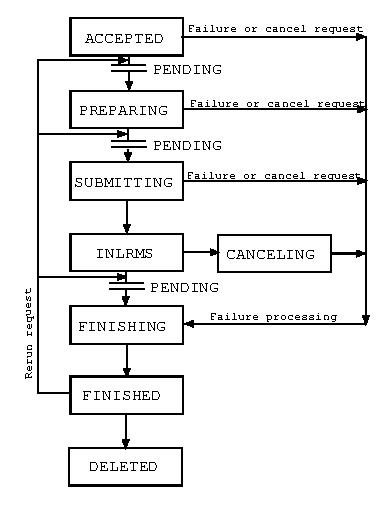
\includegraphics{pic1}
\par\end{centering}


\caption{\label{job states diagram}Job states}
\end{figure}
A user can examine the state of a job by querying the NorduGrid Information
System (IS) using the UI or any other tool. Please remember that IS
can manipulate with state names to make them more user friendly and
to combine them with states introduced by other parts of whole setup.
Another way is to access virtual informational files through GridFTP
interface or to use query metod of JCS. 

Configuration can put limits on amout of simultaneous jobs at some
states. If such limit is reached job stays in it's current state waiting
for free slot. This situation is presented by prepending current state
name with \textbf{PENDING:} status mark. 

Below is description of all actions taken by the GM at every state:

\begin{itemize}
\item \textbf{Accepted} - At this state the job has been submitted to a
CE but not processed yet. The GM will analyze the JD and move to the
next stage. If JD can not be processed the job will be canceled and
moved to the state \textbf{Finishing}.
\item \textbf{Preparing} - The input data is being gathered in the SD. The
GM is downloading files specified in the JD and waiting for files
which are supposed to be downloaded by the UI. If all files are successfully
gathered the job moves to the next state. If \textbf{any} file can't
be downloaded or it takes UI too long to upload a file - the job moves
to \textbf{Finishing} state. It is possible to put limit on number
of simultaneous \textbf{Preparing} jobs. Those jobs out of limit will
stay in previous \textbf{Accepted} state with PENDING mark. Exceptions
are jobs which has no files to be downloaded. Those are processed
out of limits.
\item \textbf{Submitting} - This is a point of interaction with \emph{Local
Resource Management System} (LRMS). At the moment PBS is supported
best and correspoding backends are provided with default installation.
The job is being submitted for execution. If the local job submission
is successful the job moves to the next state. Otherwise it moves
to \textbf{Finishing}. It is possible to limit number of jobs in \textbf{Submitting}
and following \textbf{InLRMS} states.
\item \textbf{InLRMS} - The job is queued or being executed in the LRMS.
The GM takes no actions except waiting until job finishes.
\item \textbf{Cancelling} - Necessary action to cancel job in the LRMS is
being taken.
\item \textbf{Finishing} - The output data is being processed. Specified
data files are moved to the specified SEs and are optionally registered
at RC. The user can download data files from the SD by using UI or
any other tool. All the files not specified as output files are removed
from the SD at very beginning of this state. It is possible to limit
number of simultaneous jobs in this state.
\item \textbf{Finished} - No more processing is performed by the GM. The
user can continue to download data files from the SD. The SD is kept
available for some time (default is 1 week). After that it is moved
to the state \textbf{Deleted}. The 'deletion' time can be queried
at NorduGrid Information System as attribute \texttt{nordugrid-pbs-job-sessiondirerasetime}
of \texttt{nordugrid-pbs-job}. If job was moved to \textbf{Finished}
because of failure, it may be restarted on request of client. Job
is moved to a state previous to one which failed and is assigned mark
PENDING. This is needed in order to not break the configuration limits.
Exception is a job failed in \textbf{InLRMS} state and lacking input
files specified in JD. Such job is treated like failed in \textbf{Preparing}
state.
\item \textbf{Deleted} - Job is moved to this state if user does not request
job to be cleaned. Only minimal subset of information about such job
is kept.
\end{itemize}
In the case of the failure special processing is applied to output
files. All specified output files are treated as \textbf{downloadable
by user}. No files will be moved to the SE.


\section{URLs}

The GM and it's components support following data transfer protocols
and corresponding URLs: \emph{ftp, gsiftp, http, httpg, https, se,
rc} and \emph{rls.} For more information please see {}``Protocols,
Uniform Resource Locators (URL) and extensions supported in ARC''
document \cite{urls}.


\section{\label{section: internals}Internals}


\subsection{Internal Files of the Grid Manager}

For each local UNIX user listed in the GM configuration a \textit{control
directory} exists. In this directory the GM stores information about
jobs belonging to that user. Multiple users can share the same \textit{control
directory}. To make it easier to recover in the case of failure, the
GM stores most information in files rather than in memory. All files
belonging to same job have names starting with \textbf{job.ID.} here
ID is the job identifier.

The files in the control directory and their formats are described
below:

\begin{itemize}
\item \textit{job.ID.status} - current state of the job. It contains one
word of text representing the current state of the job. Possible values
are :

\begin{itemize}
\item ACCEPTED
\item PREPARING
\item SUBMITTING
\item INLRMS
\item FINISHING
\item FINISHED
\item CANCELING
\item DELETED
\end{itemize}
\end{itemize}
See section \ref{Section: Job Flow} for a description of the various
states. Additionally each value can be prepended with a prefix {}``PENDING:''
(like PENDING:ACCEPTED, see section \ref{Section: Job Flow}). That
is used to show that the job is \emph{ready} to be moved to a next
state and it stays in a current state \emph{only} because some limits
set in configuration are exceeded.

\begin{itemize}
\item \textit{job.ID.description} - contains the RSL description of the
job.
\item \textit{job.ID.local} - information about job used by the GM. It consists
of lines of format \textit{{}``name = value''} . Not all of them
are always available. The following names are defined:

\begin{itemize}
\item \textit{subject} - user subject also known as the distinguished name
(DN)
\item \textit{starttime} - the GMT time when the job was accepted represented
in Generalized Time format of LDAP 
\item \textit{lifetime} - time period to live for the SD after job finished
in seconds
\item \textit{cleanuptime} - the GMT time when job to be removed from cluster
and SD deleted in Generalized Time format
\item \textit{notify} - email addresses and flags to send mail to about
job specified status changes
\item \textit{processtime} - the GMT time when to start processing the job
in Generalized Time format
\item \textit{exectime} - the GMT time when to start job execution in Generalized
Time format
\item \textit{expiretime} - the GMT time when credentials delegated to job
expire in Generalized Time format
\item \textit{rerun} - number of retries left to run the job
\item \textit{jobname} - name of the job as supplied by the user
\item \textit{lrms} - name of LRMS to run the job at
\item \textit{queue} - name of the queue to run the job at
\item \textit{localid} - job id in LRMS (appears only then the job is at
state \textbf{InLRMS})
\item \textit{args} - list of command-line arguments including the executable
\item \textit{downloads} - number of files to download into SD before execution
\item \textit{uploads} - number of files to upload from SD after execution
\item \textit{gmlog} - directory name which holds files containing information
about job when accessed through GridFTP interface
\item \textit{clientname} - name and ip address:port of client machine (name
is provided by user interface)
\item \textit{clientsoftware} - version of software used to submit job
\item \textit{sessiondir} - SD of job
\item \textit{failedstate} - state at which job failed (available only if
it is possible to restart job)
\item \textit{jobreport} - URL of \emph{logger service} used to keep track
of executed jobs (one requested by user)
\end{itemize}
\end{itemize}
This file is filled partially during job submission and fully when
the job moves from the \textbf{Accepted} to the \textbf{Preparing}
state.

\begin{itemize}
\item \textit{job.ID.input} - list of input files. Each line contains 2
values separated by a space. First value contains name of the file
relative to the SD. Second value is an URL or a file description.
Example:


\hspace*{1cm}\textit{input.dat gsiftp://grid.domain.org/dir/input\_12378.dat}

\textit{url} - ordinary URL for gsiftp, ftp, http, https or httpg
protocols with the addition of '\textbf{replica catalog url}' (RC
URL) and '\textbf{replica location service url}' (RLS URL).\\
Each URL can contain additional options.

\textit{file description} - {[}size]{[}.checksum].

\hspace*{1cm}\textit{size} - size of the file in bytes.

\hspace*{1cm}\textit{checksum} - checksum of the file identical to
the one produced by \textbf{\textit{cksum}} (1).

Both size and checksum can be left out. Special kind of file description
{*}.{*} is used to specify files which are \textbf{not} required to
exist.

\end{itemize}
This file is used by the '\textbf{\textit{downloader}}' utility. Files
with 'url' will be downloaded to the SD and files with 'file description'
will simply be checked to exist. Each time a new \textbf{valid} file
appears in the SD it is removed from the list and \textit{job.ID.input}
is updated. Any external tool can thus track the process of collecting
input files by checking \textit{job.ID.input.}

\begin{itemize}
\item \textit{job.ID.output} - list of output files. Each line contains
1 or 2 values separated by a space. First value is the name of the
file relative to the SD. The second value, if present, is a URL. Supported
URLs are the same as those supported by job.ID.input.
\end{itemize}
This file is used by the '\textbf{\textit{uploader}}' utility. Files
with \textit{url} will be uploaded to SE and remaining files will
be left in the SD. Each time a file is uploaded it is removed from
the list and \textit{job.ID.output} is updated. Files not mentioned
as output files are removed from the SD at the the beginning of the
\textbf{Finishing} state.

\begin{itemize}
\item \textit{job.ID.failed} - the existence of this file marks the failure
of the job. It can also contain one or more lines of text describing
the reason of failure. Failure includes the return code different
from zero of the job itself.
\item \textit{job.ID.errors} - this file contains the output produced by
external utilities like \textbf{\textit{downloader}}, \textbf{\textit{uploader}},
script for job submission to LRMS, etc on their stderr handle. Those
are not necessarily errors, but can be just useful information about
actions taken during the job processing. In case of problem include
content of that file while asking for help.
\item \textit{job.ID.diag} - information about resources used during execution
of job and other information suitable for diagnostics and statistics.
It's format is similar to that of \textit{job.ID.local}. The following
names are at least defined:

\begin{itemize}
\item \textit{nodename} - name of computing node which was used to execute
job,
\item \textit{runtimeenvironments} - used runtime environments separated
by ';',
\item \textit{exitcode} - numerical exit code of job,
\item \textit{frontend\_distribution} - name and version of operating system
distribution on frontend computer,
\item \textit{frontend\_system} - name of operating on frontend computer,
\item \textit{frontend\_subject} - subject (DN) of certificate representing
frontend computer,
\item \textit{frontend\_ca} - subject (DN) of issuer of certificate representing
frontend computer,
\end{itemize}
and other information provided by GNU \emph{time} utility. Note that
some implementation of \emph{time} insert unrequested information
in their output. Hence some lines can have broken format.

\item \textit{job.ID.proxy} -delegated GSI proxy.
\item \textit{job.ID.proxy.tmp} - temporary GSI proxy with different unx
ownership used by processes run with effective \emph{user id} different
form job owner's \emph{id}.
\end{itemize}
There are other files with names like job.ID.{*} which are created
and used by different parts of the GM. Their presence in the \textit{control
directory} can not be guaranteed and can change depending on changes
in the GM code.


\subsection{GridFTP Interface}

The GridFTP Interface to job management is implemented through GridFTP
server. The GFS is made of layer implementing GridFTP protocol and
plugins for accessing actual data. Local file access in the GFS is
implemented through plugins (shared libraries). There are 3 plugins
provided with the GFS: \textit{fileplugin.so, gaclplugin.so} and \textit{jobplugin.so}
. 

The \textit{fileplugin.so} is intended to be uses for plain file access
with the configuration senitive to user subject and is not needed
for job management interface. 

The \textit{gaclplugin.so} uses GACL (\url{http://www.gridpp.ac.uk/authz/gacl/})
to control access to local file system instead of Unix user identity.
It's also not needed for job management.

The \textit{jobplugin.so} is using information about jobs being controlled
by GM and provides access to session directories of the jobs owned
by user. It also provides an interface (virtual directory and virtual
operations) to submit, cancel, clean, renew credentials and obtain
information about the job.


\subsection{Web Service Interface}

A-REX Web Service Interface provides means to submit a description
of a computational job to a computing resource, to stage-in additional
data, to monitor and control processing of jobs, and obtain data produced
during the execution of a job. The WS Interface is built and deployed
inside Hosting Envirnoment Daemon {[}HED] infrastructure\cite{hed}.


\subsubsection{Basic Execution Service Interface}

The job submission and control interface is based on document produced
by OGF OGSA Basic Execution Services (BES) Working Group\cite{bes}.
The exchange of SOAP messages is performed over HTTPS protocol. The
BES interface is represented by two port-types - BES-Management and
BES-Factory. The former is made to control the A-REX service itself
and thus defines operations to start and stop the functionality of
the BES service. A-REX does not implement remote control of service
functionality. Hence the BES-Management port-type is not implemented.
The BES-Factory port-type provides operations to submit new jobs (to
create an activity in terms of BES) and to monitor its state. It also
has an ability to provide information about the service. A-REX fully
implements the functionality of this port-type.

For job descriptions A-REX accepts the Job Submission Description
Language (JSDL)\cite{jsdl} as defined by the OGF Job Submission Description
Language Working Group. Supported elements and extensions are described
below.


\subsubsection{Extensions to OGSA BES interface}

A-REX introduces a new operation in addition to those provided by
BES. It does that by defining its own port-type A-REX with the single
operation \emph{ChangeActivityStatus} (see Appendix D). This operation
provides a way to request simple transfers between states of jobs
being processed and corresponding actions.

\begin{itemize}
\item \emph{ChangeActivityStatus}

\begin{itemize}
\item Input

\begin{itemize}
\item \emph{ActivityStatusType OldStatus}: Description of the state the
job is supposed to be in during execution of this request. If the
current state of the job is different from the one having been given,
the operation is aborted and a fault is returned. This parameter is
optional.
\item \emph{ActivityStatusType NewStatus}: Description of the state the
job is to be put into.
\end{itemize}
\item Output

\begin{itemize}
\item \emph{ActivityStatusType NewStatus}: Description of the current state
of the job.
\end{itemize}
\item Fault(s)

\begin{itemize}
\item \emph{NotAuthorizedFault}: Indicates that client is not allowed to
do this operation.
\item \emph{InvalidActivityIdentifierFault}: There is no such job/activity.
\item \emph{CantApplyOperationToCurrentStateFault}: Requested transition
is not possible.
\end{itemize}
\end{itemize}
\end{itemize}
On result of this command, the job should be put into the requested
state. If such a procedure cannot be performed immediately then the
corresponding sequence is initiated and fault OperationWillBeAppliedEventuallyFault
will be returned.

Since BES allows implementators to extend their initial activity states
with additional sub-states, A-REX defines a set of sub-states of activity
processing in addition to those defined by the BES, as listed in Table
\ref{tab:Job-states-definitions}.

%
\begin{table}

\caption{\label{tab:Job-states-definitions}Job states definitions and mappings}

\begin{tabular}{|c|c|>{\raggedright}p{10cm}|}
\hline 
Applicable BES State&
ARC Sub-state&
\multicolumn{1}{c|}{Description}\tabularnewline
\hline
\hline 
\renewcommand{\multirowsetup}{\centering}\multirow{2}{2cm}{Pending}&
Accepting&
Job is in the process of being submitted\tabularnewline
\cline{2-2} \cline{3-3} 
\multicolumn{1}{|c|}{}&
Accepted&
Job was submitted\tabularnewline
\hline 
\renewcommand{\multirowsetup}{\centering}\multirow{7}{2cm}{Running}&
Preparing&
Stage-in process is going on\tabularnewline
\cline{2-2} \cline{3-3} 
\multicolumn{1}{|c|}{}&
Prepared&
Stage-in process has finished\tabularnewline
\cline{2-2} \cline{3-3} 
\multicolumn{1}{|c|}{}&
Submitting&
Communication with local batch system is in process\tabularnewline
\cline{2-2} \cline{3-3} 
\multicolumn{1}{|c|}{}&
Executing&
Job is being executed in local batch system\tabularnewline
\cline{2-2} \cline{3-3} 
\multicolumn{1}{|c|}{}&
Killing&
Communication with local batch system to terminate execution is in
process\tabularnewline
\cline{2-2} \cline{3-3} 
\multicolumn{1}{|c|}{}&
Executed&
Job execution in local batch system has finished\tabularnewline
\cline{2-2} \cline{3-3} 
\multicolumn{1}{|c|}{}&
Finishing&
Stage-out process is going on\tabularnewline
\hline 
Cancelled&
Failed&
There was a failure during execution\tabularnewline
\cline{1-1} 
Failed&
\multicolumn{1}{c|}{}&
\multicolumn{1}{l|}{}\tabularnewline
\hline 
All&
Pending&
Job is prevented from going to the next state due to some internal
limits; this sub-state appears in parallel with other sub-states\tabularnewline
\hline 
All&
Held&
Job processing is suspended on client request; this sub-state appears
in parallel with other sub-states\tabularnewline
\hline
\end{tabular}
\end{table}



\subsubsection{Delegation Interface}

ARC service interfaces optionally offer a sub-interface, called the
Delegation Interface (see Appendix E). This is a common purpose interface
to be used by ARC services which accept delegated credentials from
clients. The Delegation Interface implements two operations: initiatialization
of credentials delegation (DelegateCredentialsInit) and update/renewal
of credentials (UpdateCredentials).

\begin{itemize}
\item \emph{DelegateCredentialsInit} operation - this operation performs
the first half of the credentials delegation sequence.

\begin{itemize}
\item Input

\begin{itemize}
\item None. On this request the service generates a pair of \emph{public}
and private keys. The public key is then sent to the client in response.
\end{itemize}
\item Output(s)

\begin{itemize}
\item \emph{TokenRequestType TokenRequest}: Contains the public key generated
by the service as a Value element. It also provides an identifier
in the Id element which should be used to refer to the corresponding
private key.
\end{itemize}
\item Fault(s)

\begin{itemize}
\item \emph{UnsupportedFault}: Indicates that the service does not support
this operation despite supporting the port-type.
\item \emph{ProcessingFault}: Internal problems during generation of the
token.
\end{itemize}
\end{itemize}
\item \emph{UpdateCredentials} operation - this operation makes it possible
to update the content of delegated credentials (like in the case of
credentials being renewed) unrelated to other operations of the service.

\begin{itemize}
\item Input

\begin{itemize}
\item \emph{DelegatedTokenType DelegatedToken}: Contains an X509 proxy certificate
based on the public key from the DelegateCredentialsInit signed by
the user's proxy certificate. Also includes the Id element which identifies
the private key stored at the service side associated with these credentials.
The reference element refers to the object which these credentials
should be applied to in a way specific to the service. The same element
must also be used for delegating credentials as part of other operations
on service.
\end{itemize}
\item Output(s)

\begin{itemize}
\item None.
\end{itemize}
\item Fault(s)

\begin{itemize}
\item \emph{UnsupportedFault}: Indicates that service does not support this
operation despite supporting the port-type.
\item \emph{ProcessingFault}: Internal problems during generation of the
token.
\end{itemize}
\end{itemize}
\end{itemize}
Additionally, A-Rex Web Service Interface allows delegation to be
performed as part of the \emph{CreateActivity} operation of the BES-Factory
port-type. For this it accepts the element \emph{DelegatedCredentials}
inside the \emph{CreateActivity} element. The \emph{Id} element of
\emph{DelegatedCredentials} must contain an identifier obtained in
response to the previous \emph{DelegateCredentialsInit} operation.


\subsubsection{Local Information Description Interface}

The A-REX implements the Local Information Description Interface (LIDI)
interface being common for all ARC services. This interface is based
on OASIS Web Services Resource Properties specification\cite{wsrf-rp}.
Information about resources and maintained activities/jobs are represented
in a \emph{WS-Resource Properties} informational XML document. The
document type is defined in the A-Rex WSDL as a \emph{ResourceInformationDocumentType}.
It contains the following elements/resources:

\begin{lyxlist}{00.00.0000}
\item [{\emph{BESFactory}}] - collection of BES Factory attributes as defined
in the BES specifications.
\item [{\emph{Glue2Resource}}] \emph{-} description of a computation resource
that uses Glue2 schema. This one is going to be specified after the
Glue2 XML bindings will be available.
\item [{\emph{Activities}}] \emph{-} list of maintained activities. Each
activity contains an identifier (\emph{ActivityIdentifier}), BES (\emph{ActivityDocument})
and Glue2 (\emph{Glue2Job}) descriptions of the activity.
\end{lyxlist}
All information can be accessed either through requests on particular
resources or through XPath queries using WS-Resource Properties operations.


\subsubsection{Supported JSDL elements}

A-REX supports the following elements from the JSDL version 1.0 specification\cite{jsdl}
including POSIX Applications extension:

\begin{lyxlist}{00.00.0000}
\item [{\emph{JobName}}] \emph{-} name of the job as assigned by the user.
\item [{\emph{Executable}\ (POSIX)}] - name of the executable file.
\item [{\emph{Argument}\ (POSIX)}] - arguments the executable will be
launched with.
\item [{\emph{DataStaging}}]~

\begin{lyxlist}{00.00.0000}
\item [{Filename}] - name of the data file on the executing node.
\item [{\emph{Source}}] - source where the file will be taken from before
execution.
\item [{\emph{Target}}] \emph{-} destination the file will be delivered
to after execution.
\end{lyxlist}
\item [{\emph{Input}\,\ (POSIX)}] - file to be used as standard input
for the executable.
\item [{\emph{Output}\ (POSIX)}] - file to be used as standard output
for the executable.
\item [{\emph{Error}\ (POSIX)}] - file to be used as standard error for
the executable.
\item [{\emph{MemoryLimit}\ (POSIX)}] - amount of physical memory needed
for execution.
\item [{\emph{TotalPhysicalMemory}}] - same as MemoryLimit.
\item [{\emph{IndividualPhysicalMemory}}] - same as MemoryLimit.
\item [{\emph{CPUTimeLimit}\ (POSIX)}] - maximal amount of CPU time needed
for execution.
\item [{\emph{TotalCPUTime}}] - same as CPUTimeLimit.
\item [{\emph{IndividualCPUTime}}] - same as CPUTimeLimit.
\item [{\emph{WallTimeLimit}\ (POSIX)}] - amount of clock time needed
for execution.
\item [{\emph{TotalCPUCount}}] \emph{-} number of CPUs needed for execution.
\item [{\emph{IndividualCPUCount}}] - same as TotalCPUCount.
\end{lyxlist}

\subsubsection{ARC-specific JSDL Extensions}

A-REX accepts JSDL documents having the following additional elements
(see Appendix F):

\begin{lyxlist}{00.00.0000}
\item [{\emph{IsExecutable}}] \emph{-} marks file to become executable
after being delivered to the computing resource.
\item [{\emph{RunTimeEnvironment}}] - specifies the name of the Runtime
Environment needed for job execution.
\item [{\emph{Middleware}}] - request for specific middleware on the computing
resource frontend.
\item [{\emph{RemoteLogging}}] \emph{-} destination for the usage record
report of the executed job.
\item [{\emph{LocalLogging}}] - name for the virtual directory available
through job interface and containing various debug information about
job execution.
\item [{\emph{AccessControl}}] - ACL expression which describes the identities
of those clients who are allowed to perform operations on this job.
\item [{\emph{Notify}}] - Email destination for notification of job state
changes.
\item [{\emph{SessionLifeTime}}] - duration for the directory containing
job-related files to exist after the job finished executing.
\item [{\emph{JoinOutputs}}] - specifies if standard output and standard
error channels must be merged.
\item [{\emph{Reruns}}] \emph{-} defines how many times a job is allowed
to rerun in case of failure.
\item [{\emph{CredentialServer}}] \emph{-} URL of MyProxy service which
may be used for renewing the expired delegated job credentials.
\item [{\emph{CandidateTarget}}] \emph{-} specifies host name and queue
of a computing resource.
\end{lyxlist}

\section{Cache\label{sec:cache}}

The GM can cache input files. Caching is enabled if corresponding
command is present in configuration file. The GM does not cache files
marked as executable in job. Caching can also be explicitly turned
off by user for each file by using \textit{cache=no} option in URL
(for URL options read {}``Protocols, Uniform Resource Locators (URL)
and extensions supported in ARC'' \cite{urls}). The disc space occupied
by cache is controlled by removing unused files. For more information
look in section \ref{SubSection: ConfigFile}.


\subsection{Structure}

Cache directory contains plain files. Those are

\begin{itemize}
\item \textit{list} - stores names of the files (8 digit numbers) and corresponding
URLs delimited by blank space. Each pair is delimited by some amount
of \textbackslash{}0 codes. Also creation and expiration times are
stored if available
\item \textit{old} - stores URLs which have been removed from cache. Records
are delimited by some amount of \textbackslash{}0 codes and are meant
to be removed by some external routine.
\item \textit{new} - stores URLs which have been added to cache. Records
are delimited by some amount of \textbackslash{}0 codes and are removed
when corresponding files are removed from cache. They can also be
handled by some external routines. Every time record is added to \emph{old}
it is removed from \emph{new}.
\item \textit{statistics} - consists of strings containing \emph{name=value}
. Following names are defined:

\begin{itemize}
\item \textit{hardsize} -size of file system for storing cached data
\item \textit{hardfree} - amount of disc space available on that file system
\item \textit{softsize} - if cache exceeds this size files are started being
removed 
\item \textit{softfree} - space left till softsize (can be negative)
\item \textit{claimed} - space used by files claimed by running jobs
\item \textit{unclaimed} - space used by files not being currently used
by any job
\end{itemize}
\item \textit{\#\#\#\#\#\#\#\#.info} - stores state of file (\textit{\#\#\#\#\#\#\#\#}
stands for 8 digits). State is represented by one character:\\
\textit{c} - just created, content is empty.\\
\textit{f} - failed to download (treated same as 'c').\\
\textit{r} - ready to be used, content is valid.\\
\textit{d} - being downloaded. 'd' is followed by identifier of application/job
downloading that file. During content's download this file has write
lock set.
\item \textit{\#\#\#\#\#\#\#\#.claim} - stores list of identifiers of applications/jobs
using this file. Identifiers are stored one per line.
\item \textit{\#\#\#\#\#\#\#\#} - files storing content of corresponding
URL. These can be stored in separate directory.
\end{itemize}
Files \textit{list, old , new} and \textit{\#\#\#\#\#\#\#\#.info}
has to be stored on filesystem which has support for files' locking.


\subsection{How it works}

If job requests input file, which can/allowed to be cached, it is
stored in cache directory instead and soft-link is created in the
SD, pointing to that file. Or file can be stored in cache and then
copied to the SD. Last option is more secure and hence advised.

Before downloading file the GM tries to determine it's size and to
preallocate space in cache directory, by writing file of same size.
If that fails (file system has no more space), it tries to remove
oldest cache files, which are not being used by any job. That means
\textbf{hard limit of cache size is space available at file-system}.
In case cache gets full and it is impossible to free any space, download
fails and is retried without using cache.

Before giving access to already cached file the GM contacts initial
file source to check if user is allowed to do that if protocols allows
to do that.

Also file creation or validity times are checked to make sure cached
file is fresh enough. If it is impossible to obtain creation and invalidation
times for file it is invalidated 24 hours after downloaded.

Also the GM checks cache periodically. If used space exceeds high
water-mark given in configuration file (\emph{softsize}) it tries
to remove oldest unused files to reduce size to low water-mark. This
sets soft limit of cache size.

There are 2 kinds of caches supported. Files in \textit{private} cache
are owned by Unix user to which grid user is mapped. Those files are
readable only by that particular Unix user. Another kind of cache
is \textit{shared}. Files are owned by Unix user who started GM and
are readable by everyone.


\section{Files and directories\label{sec:files and directories}}


\subsection{Modules}

The GM consists of few separate executable modules. Those are:

\begin{itemize}
\item \textit{grid-manager} - Main module. It is responsible for processing
the job, moving it through states, running other modules.
\item \textit{downloader} - This is a module responsible for gathering input
files in the SD. It processes the \textit{job.ID.input} file and updates
it.
\item \textit{uploader} - This module is responsible for delivering output
files to the specified SEs and registration at the RC. It processes
and updates the \textit{job.ID.output} file.
\item \emph{cache-register} - Utility to register cached data into Indexing
Services like RC and RLS. It reads and modifies cache informational
files \emph{old} and \emph{new} \ref{sec:cache}. Configuration is
read directly from the GM's configuration file \ref{SubSection: ConfigFile}.
It is run by the GM every 5 minutes.
\item \emph{frontend-info-collector} - Utility to gather information about
frontend and to put it into \emph{job.ID.diag} file.
\item \emph{gm-kick} - Sends signal to the GM though FIFO file to wake it
up. It's used to increase responsiveness of GM.
\end{itemize}
Following modules are always run under Unix account to which user
is mapped.

\begin{itemize}
\item \textit{smtp-send.sh} and \textit{smtp-send} - These are the modules
responsible for sending e-mail notifications to the user. The format
of the mail messages can be easily changed by editing the simple shell
script \textit{smtp-send.sh}. 
\item \textit{submit-{*}-job} - Here {*} stands for the name of the LRMS.
Curently supported LRMS are PBS/Torque, Condor and SGE. Also \emph{fork}
pseudo-LRMS is supported for testing purposes. This module is responsible
for the job submission to the LRMS.
\item \textit{cancel-{*}-job} - This one is for canceling the job, which
was submitted to LRMS.
\item \textit{scan-{*}-job} -This shell script is responsible for notifying
the GM about completion of the job. It's implementation for PBS system
uses server logs to extract information about jobs. If logs are not
available it uses less reliable \emph{qstat} command for that. other
backends use different techniques.
\end{itemize}
Also there is administrator utility:

\begin{itemize}
\item \textit{gm-jobs} - prints list of jobs available on cluster and amount
of jobs in every state.\\
\hspace*{0.5cm}gm-jobs {[}-h] {[}-l] {[}-u uid] {[}-U name]\\
\hspace*{0.5cm}-l-l - print more information about each job,\\
\hspace*{0.5cm}-l-u - pretend utility is run by user with id \emph{uid},\\
\hspace*{0.5cm}-l-l - pretend utility is run by user with name \emph{name}.
\end{itemize}
GM comes with plugins useable for various authorization purposes (see
for example description of \emph{authplugin} command below):

\begin{itemize}
\item \textit{inputcheck} - checks if all input files specified in job description
are downloadable.\\
\hspace*{0.5cm}inputcheck {[}-h] {[}-d debug\_level] RSL\_fle {[}proxy\_file]\\
\hspace*{0.5cm}-lRSL\_file -file with job description,\\
\hspace*{0.5cm}-lproxy\_file - credentials proxy.
\item \textit{lcas} - executes LCAS plugins on credentials and returns 0
if authorization passed.\\
\hspace*{0.5cm} lcas credentials description {[}library {[}db {[}directory]]]\\
\hspace*{0.5cm}-lcredentials - path to file with credentials to authorize,\\
\hspace*{0.5cm}-ldescription - path to file with job description,\\
\hspace*{0.5cm}-llibrary - path to LCAS library (full or relative
to LCAS directory),\\
\hspace*{0.5cm}-ldb - path to LCAS DB file (full or relative to LCAS
directory),\\
\hspace*{0.5cm}-ldirectory - LCAS directory.
\end{itemize}

\subsection{Directories}

The GM is installed into a single installation point referred as \$NORDUGRID\_LOCATION
and following sub-directories are used:

\begin{LyXParagraphLeftIndent}{1cm}
\$NORDUGRID\_LOCATION/bin - tools

\$NORDUGRID\_LOCATION/libexec - program modules used by GM

\$NORDUGRID\_LOCATION/etc - configuration files, deprecated, central
configuration file is used by deault

\$NORDUGRID\_LOCATION/sbin - daemons

\$NORDUGRID\_LOCATION/lib - gridftp server's plugins and API libraries

The GM also uses following directories:

\end{LyXParagraphLeftIndent}
\begin{itemize}
\item \textit{session root directory} - In this directory the SD is created.
It can be multiple directories for the various users specified in
the configuration file.\\
There are 2 processes which need to have a permissions to create new
files and directories in it. Those are GM and GFS. \\
If any of those processes processes are run under dedicated user account,
that account need full permissions in the \textit{session root directory}.\\
If those processes are run under \emph{root} account make sure \textit{session
root directory} is not on filesystem which limits capabilities of
\emph{root} user. For example NFS with \emph{root\_squash} option.\\
If there is need to run processes under \emph{root} account (to run
jobs in LRMS under different users' accounts) but there is no way
to provide suitable \textit{session root directory} use \emph{norootpower}
command in configuration of the GM. In that case GM and GFS will use
identity of local user to which Grid identity is mapped to access
\textit{session root directory}. Hence those users will need full
access there.\\
The GM creates SD with proper ownership and permissions for local
identity used to run job. Some filesystems require \emph{executable}
permissions on \textit{session root directory} to be set for local
identity in order to access any file or subdirectory there.\\
This directory should also be shared among cluster nodes in order
for job to access input files. Or internal means of LRMS must be used
to transfer files to executing node. For more see section \ref{sub:LRMS}.
\item \textit{control directory} - In this directory the SD stores an information
about the accepted jobs. Both GM and GFS processes must have full
permissions there.\\
Also subdirectory called \textit{log} is created there. It is used
to accumulate information about started and finished jobs. This information
is periodically sent to the \emph{logger service}.
\end{itemize}

\section{Configuration}


\subsection{\label{SubSection: ConfigFile}Configuration of the Grid Manager}

The GM configuration is done through single configuration file. Historically
GM supports 2 kinds of configuration files. For old one it looks at
following places:

\begin{itemize}
\item \textit{\$NORDUGRID\_LOCATION/etc/grid-manager.conf}
\item \textit{/etc/grid-manager.conf}
\end{itemize}
And for new one in 

\begin{itemize}
\item \textit{/etc/arc.conf}
\end{itemize}
The old configuration file consists of empty lines, lines containing
comment (line starts from \#) or configuration commands. Blank spaces
in arguments must be escaped using '\textbackslash{}' or arguments
must be enclosed in '\char`\"{}'. Command line starts from command
followed by arguments separated from command and between them by spaces.

The new configuration file can also contain empty lines and comments
starting from \#. It is separated into sections. Each sections starts
from string containing \emph{}

\begin{itemize}
\item \emph{{[}section name/subsection name/subsubsection name]}. 
\end{itemize}
Each section continues till next section of end of file. One configuration
file can have commands for multiple services/modules/programs. Each
service get it's own section named after it. The GM uses section \emph{{[}grid-manager]}.
Some services can make use of multiple subsections to reflect their
internal modular structure. Commands in section \emph{{[}common]}
apply to all services. Command lines have format 

\begin{itemize}
\item \emph{name=''arguments string''.}
\end{itemize}
Names are same as in old configuration file. The \emph{argument string}
consists of same arguments as in old format. And they must obey same
rules.

Both files support almost same commands. Following commands are defined
(examples are given for new format):

\noindent Global commads (those which affect global parameters of
the GM and affect all serviced users, also described in \cite{config}):

\begin{itemize}
\item \textbf{\textit{daemon}}\textit{=yes|no} - specifies whether the GM
should go to background after started. Defaults to \emph{yes}.
\item \textbf{\textit{logfile}}\textit{={[}path]} - specifies name of file
for logging debug/informational output. Defaults to \emph{/dev/null}
for daemon mode and \emph{stderr} for foreground mode.
\item \textbf{\textit{user}}\textit{={[}uid{[}:gid]]} - specifies user id
(and optionally group id) to which the GM must switch after reading
configuration. Defaults to \emph{not switch}.
\item \textbf{\textit{pidfile}}\textit{={[}path]} - specifies file where
id if GM process will be stored. Defaults to \emph{not write}.
\item \textbf{\textit{debug}}\textit{=number} - specifies level of debug
information. More information is printed for higher levels. Currently
highest effective number is 3 and lowest 0. Defaults to 2.
\end{itemize}
All commands above are generic for every daemon-enabled server in
ARC NorduGrid toolkit (like GFS and HTTPSD).

\begin{itemize}
\item \textbf{\textit{joblog}}\textit{={[}path]} - specifies where to store
log file containing information about started and finished jobs.
\item \textbf{\textit{jobreport}}\textit{={[}URL ... number]} - specifies
that GM has to report information about jobs being processed (started,
finished) to centralized service running at given \textit{URL}. Multiple
entries and multiple URLs are allowed. \textit{number} specifies how
long old records have to be kept if failed to be reported. That time
is in days. Last specified value becomes effective.
\item \textbf{\textit{securetransfer}}\textit{=yes|no} - specifies whether
to use encryption while transferring data. Currently works for GridFTP
only. Default is no. It is overridden by value specified in URL options.
\item \textbf{\textit{localtransfer}}\textit{=yes|no} - specifies whether
to pass file downloading/uploading task to computing node. If set
to yes the GM won't download/upload files. Instead it composes script
submitted to LRMS in way to make it do that. This requires installation
of GM and Globus to be accessible from computing nodes and environment
variables GLOBUS\_LOCATION and NORDUGRID\_LOCATION to be set accordingly.
Default is no.
\item \textbf{\textit{maxjobs}}\textit{={[}max\_processed\_jobs {[}max\_running\_jobs]]}
- specifies maximum number of jobs being processed by the GM at different
stages:\\
\textit{max\_processed\_jobs} - maximal amount of jobs being processed
by GM. This does not limit amount of jobs, which can be suNOTE:bmitted
to cluster\\
\textit{max\_running jobs} - maximal amount of jobs passed to Local
Resource Management System\\
Missing value or -1 means no limit.
\item \textbf{\textit{maxlod}}\textit{={[}max\_frontend\_jobs {[}emergency\_frontend\_jobs
{[}max\_transferred\_files]]]} - specifies maximum load caused by
jobs being processed on frontend:\\
\textit{max\_frontend\_jobs} - maximal amount of jobs heavily using
resources of frontend (applied before moving job to PREPARING and
FINISHING states)\textit{}\\
\textit{emergency\_frontend\_jobs} - if limit of \textit{max\_frontend\_jobs}
is used only by PREPARING or by FINISHING jobs aforementioned number
of jobs can be moved to another state .This is used to avoid case
then jobs can't finish due to big amount of recently submitted jobs.\textit{}\\
\textit{max\_transfered\_files} - maximal number of files being transfered
in parallel by every job. Used to decrease load on not so powerful
frontends.\\
Missing value or -1 means no limit.
\item \textbf{\textit{wakeupperiod}}\textit{=time} - specifies how often
for external changes are performed (like new arrived job, job finished
in LRMS, etc.). \textit{time} is a minimal time period specified in
seconds. Default is 3 minutes.
\item \textbf{\textit{cacheregistration}}\textit{=yes|no} - enables or disables
registration of cache data into Indexing Services like RC or RLS.
The default is \emph{no}. Only files dowmloaded through \emph{meta-url}
are registred. Registration is done to same service used for obtaining
information about file. For this opeartion credentials of the GM (host
key and certificate) are used. If required new files storage location
is registered at Indexing Service with quasi-url \emph{cache://hostname/}
and name \emph{hostname:cache} .
\item \textbf{\textit{authplugin}}\textit{=state options plugin} - specifies
\emph{plugin} (external executable) to be run every time job is going
to switch to \emph{state}. Following states are allowed: ACCEPTED,
PREPARING, SUBMIT, FINISHING, FINISHED and DELETED. If exit code is
not 0 job is canceled by default. \textit{Options} consist of \textit{name}=\textit{value}
pairs separated by a comma. Following \textit{name}s are supported:\\
\textit{timeout} - specifies how long in seconds execution of the
plugin allowed to last (mandatory, {}``\textit{timeout=}{}`` can
be skipped for backward compatibility).\\
\textit{onsuccess}, \textit{onfailure} and \textit{ontimeout} - defines
action taken in each case (\textit{onsuccess} happens if exit code
is 0). Possible actions are:\\
\textit{pass} - continue execution,\\
\textit{log} - write information about result into logfile and continue
execution,\\
\textit{fail} - write information about result into logfile and cancel
job.
\item \textbf{\textit{localcred}}\textit{=timeout plugin} - specifies \emph{plugin}
(external executable or function in shared library) to be run every
time job has to do something on behalf of local user. Execution of
\emph{plugin} may not last longer than \emph{timeout} seconds. If
\emph{plugin} looks like \emph{function@path} then function \emph{int
function(char{*},char{*},char{*},...)} from shared library \emph{path}
is called (\emph{timeout} is not functional in that case). If exit
code is not 0 current operation will fail.
\item \textbf{\textit{norootpower}}\textit{=yes/no} - if set to yes all
processes involved in job management will use local identity of a
user to which Grid identity is mapped in order to access filesystem
at path specified in \textbf{\textit{session}} command (see below).
Sometimes this may involve running temporary external process.
\item \textbf{\textit{allowsubmit}}\textit{={[}group ...]} - list of authorization
groups of users allowed to submit new jobs while \char`\"{}allownew=no\char`\"{}
is active in \emph{jobplugin.so} configuration (see below in section
\ref{subsec: configfile of the gfs}). Multiple commands are allowed.
\item \textbf{\textit{speedcontrol}}\textit{=min\_speed min\_time min\_average\_speed
max\_inactivity} - specifies how long/slow data fransfer is allowed
to take place. Transfer is canceled if transfer rate (bytes per second)
is lower than \emph{min\_speed} for at least \emph{min\_time} seconds,
or if average rate is lower than \emph{min\_average\_speed}, or no
data is receved for longer than \textit{max\_inactivity} seconds.
\item \textbf{\textit{copyurl}}\textit{=template replacement} - specifies
that URLs, starting from template should be accessed in a different
way (most probably Unix open). The \textit{template} part of the URL
will be replaced with \textit{replacement.} \textit{replacement} can
be either URL or local path starting from '/'. It is advisable to
end template with '/'.
\item \textbf{\textit{linkurl}}\textit{=template replacement {[}node\_path]}
- mostly identical to \textit{copyurl} but file won't be copied. Instead
soft-link will be created. \textit{replacement} specifies the way
to access the file from the frontend, and is used to check permissions.
The \textit{node\_path} specifies how the file can be accessed from
computing nodes, and will be used for soft-link creation. If \textit{node\_path}
is missing - \textit{local\_path} will be used instead. Both \textit{node\_path}
and \textit{replacement} should not be URLs.


NOTE: URLs which fit into \textit{copyurl} or \textit{linkurl} are
treated as more easily accessible than other URLs. That means if GM
has to choose between few URLs from which should it download input
file, these will be tried first.

\end{itemize}
\noindent Per UNIX user commands:

\begin{itemize}
\item \textbf{\textit{mail}}\textit{=e-mail\_address} - specifies an email
address \textbf{from} which the notification mails are sent.
\item \textbf{\textit{defaultttl}}\textit{=ttl {[}ttr]} - specifies the
time in seconds for the SD to be available after job finished (\emph{ttl})
and after job was deleted (\emph{ttr}) due to \emph{ttl}. Defaults
are 7days for \emph{ttl} and 30 days for \emph{ttr}.
\item \textbf{\textit{defaultlrms}}\textit{=default\_lrms\_name default\_queue\_name}
- specifies names for the LRMS and queue. Queue name can also be specified
in the JD (currently it is not allowed to override used LRMS by using
JD). In new configuration file this command is called \textbf{\textit{lrms}}.
\item \textbf{\textit{session}}\textit{=path} - specifies path to the directory
in which the SD is created. If the path is {*} the default one is
used - \textit{\$HOME/.jobs} . In new configuration file this command
is called \textbf{\textit{sessiondir}}.
\item \textbf{\textit{cache}}\textit{dir=path {[}link\_path]} - specifies
the directory to store cached data. Empty \emph{path} disables caching.
Default is not to cache data. Optional \textit{link\_path} specifies
the path at which cache is accessible at computing nodes. If \textit{link\_path}
is set to '.' files are not soft-linked, but copied to session directory.
In old configuration file this command is called \textbf{\textit{cache}}.
\item \textbf{\textit{privatecache}}\textit{=path {[}link\_path]} - same
as \textit{cache} command, but cache belongs (owned) to user. For
shared caches use 'cache'.
\item \textbf{\textit{cachedata}}\textit{=path} - allows to specify separate
place to store cache files containing data itself. This can be useful
in case of big data storage available only on NSF server which does
not support file locking. If command or \textit{path} is missing -
default is to store data at place specified in \textit{cache} or \textit{privatecache}
command, together with control files. 
\item \textbf{\textit{cachesize}}\textit{=high\_mark {[}low\_mark]} - specifies
high and low water-mark for space used by cache. Values are specified
in bytes. Both \textit{high\_mark} and \textit{low\_mark} can be negative
values. In that case corresponding positive value means space left
on filesystem. If \textit{low\_mark} is omitted it becomes equal to
\textit{high\_mark}. By default this feature is turned off. To turn
it off explicitly \textit{cachesize} without parameters should be
specified. If turned off cache will grow up till it fills whole file
system.
\item \textbf{\textit{maxrerun}}\textit{=number} - specifies maximal number
of times job will be allowed to rerun after it failed in LRMS. Default
value is 2. This only specifies a upper limit. Actual number is provided
in job description and defaults to 0.
\end{itemize}
All per-user commands should be put before \textit{control} command
which initiates serviced user.

\begin{itemize}
\item \textbf{\textit{control}}\textit{=path username {[}username {[}...]]}
- This option initiates UNIX user as being serviced by the GM. \textit{path}
refers to the control directory (see section \ref{section: internals}
for the description of control directory). If the path is {*} the
default one is used - \$HOME/.jobstatus . \textit{username} stands
for UNIX name of the local user. Multiple names can be specified.
If the name is {*} it is substituted by all names found in file /etc/grid-security/grid-mapfile
(for the format of this file one should study the Globus project \cite{globus}).\\
Also the special name '.'(dot) can be used. Corresponding control
directory will be used for \textbf{any} user. This option should be
the last one in the configuration file. In new configuration file
command \textbf{\textit{controldir}}\textit{=path} is also available.
It uses special username '.' and is always executed last independent
of placement in file.
\item \textbf{\textit{helper}}\textit{=username command {[}argument {[}argument
{[}...]]]} - associates external program with the local UNIX user.
This program will be kept running under account of the specified user.
\textit{username} stands for the name of the user. Special names can
be used: '{*}' - all names from /etc/grid-security/grid-mapfile, '.'
- root user. The user should be already configured with \textit{control}
option (except root, who is always configured). \textit{command} is
an executable and \textit{argument}s are passed as arguments to it.
\end{itemize}
Following are global commands supported only in new configuration
file. Most of them are specific to underlying LRMS (PBS in this case)
and are passed in environment variables if old configuration file
is used.

\begin{itemize}
\item \textbf{\textit{pbs\_bin\_path}}\textit{=path} - path to directory
which contains PBS commands.
\item \textbf{\textit{pbs\_log\_path}}\textit{=path} - path to directory
with PBS server's log files.
\item \textbf{\textit{gnu\_time}}\textit{=path} - path to \emph{time} utility.
\item \textbf{\textit{tmpdir}}\textit{=path} - path to directory for temporary
files.
\item \textbf{\textit{runtimedir}}\textit{=path} - path to directory which
contains \emph{runtimenvironment} scripts.
\item \textbf{\textit{shared\_filesystem}}\textit{=yes|no} - if compiting
nodes have an access to session directory through a shared filesystem
like NFS. Corresponds to an environement variable RUNTIME\_NODE\_SEES\_FRONTEND.
\item \textbf{\textit{nodename}}\textit{=command} - command to obtain hostname
of computing node.
\item \textbf{\textit{scratchdir}}\textit{=path} - path on computing node
where to move session directory before execution.
\item \textbf{\textit{shared\_scratch}}\textit{=path} - path on frontend
where \textbf{\textit{scratchdir}} can be found.
\item \textbf{\textit{nodename}}\textit{=command} - command to obtain hostname
of computing node.
\end{itemize}
In the command arguments (paths, executables, ...) following substitutions
can be used:

\begin{lyxlist}{00.00.0000}
\item [{\%R}] - session root - see command \emph{session}
\item [{\%C}] - control dir - see command \emph{control}
\item [{\%U}] - username
\item [{\%u}] - userid - numerical
\item [{\%g}] - groupid - numerical
\item [{\%H}] - home dir - home specified in /etc/passwd
\item [{\%Q}] - default queue - look command 'defaultlrms'
\item [{\%L}] - default lrms - look command 'defaultlrms'
\item [{\%W}] - installation path - \$\{NORDUGRID\_LOCATION\}
\item [{\%G}] - globus path - \$\{GLOBUS\_LOCATION\}
\item [{\%c}] - list of all control directories
\item [{\%I}] - job's ID (for plugins only, substituted in runtime)
\item [{\%S}] - job's state (for \emph{authplugin} plugins only, substituted
in runtime)
\item [{\%O}] - reason (for \emph{localcred} plugins only, substituted
in runtime).\\
Possible reasons are:

\begin{lyxlist}{00.00.0000}
\item [{new}] - new job, new credentials
\item [{renew}] - old job, new credentials
\item [{write}] - write/delete file, create/delete directory (through gridftp)
\item [{read}] - read file, directory, etc. (through gridftp)
\item [{extern}] - call external program (grid-manager)
\end{lyxlist}
\end{lyxlist}
Some configuration parameters can be specified from command line while
starting the GM:

\emph{grid-manager {[}-h] {[}-C level] {[}-d level] {[}-c path] {[}-F]
{[}-U uid{[}:gid]] {[}-L path] {[}-P path]}\\
\hspace*{0.5cm}\emph{-h} - short help,\\
\hspace*{0.5cm}\emph{-d} - debug level,\\
\hspace*{0.5cm}\emph{-L} - name log file (overwrites value in configuration
file),\\
\hspace*{0.5cm}\emph{-P} - name for file containing process id (overwrites
value in configuration file),\\
\hspace*{0.5cm}\emph{-U} - user and gropu id to use for running daemon,\\
\hspace*{0.5cm}\emph{-F} - do not make process daemon,\\
\hspace*{0.5cm}\emph{-c} - name od configuration file,\\
\hspace*{0.5cm}\emph{-C} - remove old information before starting:
1- remove finished jobs, 2 - remove active jobs too, 3- also remove
everything that looks like junk.\\



\subsection{\label{subsec: configfile of the gfs}Configuration of the GridFTP
Server}

Default location of the GFS configuration file is \textit{/etc/arc.conf}
or \textit{\$NORDUGRID\_LOCATION/etc/gridftpd.conf}. Format of these
configuration files is similar to that of the GM. It also supports
generic commands described at the beginning of previous section \ref{SubSection: ConfigFile}.
In the new format sections {[}common] and {[}gridftpd] are used. Commands
specific to the GFS are described below.

\begin{itemize}
\item \textbf{\textit{port}}\textit{=number} - specifies TCP/IP port number.
Default is 2811.
\item \textbf{\textit{include}}\textit{=path} - include contents of another
file. Generic commands can't be specified there.
\item \textbf{\textit{encryption}}\textit{=yes|no} - specifies if server
will allow data transfer to be encrypted. Default is yes.
\item \textbf{\textit{pluginpath}}\textit{=path} - specifies the path where
plugin libraries are installed
\item \textbf{\textit{allowunknown}}\textit{=yes|no} - if set to \emph{yes}
clients are not checked agains grid-mapfile. Hence only access rules
specified in this configuration file will be applied.
\item \textbf{\textit{firewall}}\textit{=hostname} - use IP address of the
\textit{hostname} in response to PASV command instead of IP address
of a network interface of computer. You can write IP address directly
instead of \textit{hostname}. This command may be if server is situated
behind NAT.
\item \textbf{\textit{unixgroup}}\textit{=group rule} - define local UNIX
user and optionally UNIX group to which user belonging to specified
authorization \textit{group} is mapped (see Section \ref{sub:Authorization}
for definition of group). Local names are obtained from specified
\textit{rule}. If specified rule could not produce any mapping, next
command is used. Mapping stops at first matched rule. Following rules
are supported:

\begin{itemize}
\item \textbf{\textit{mapfile}} \textit{file} - user's subject is matched
against list of subjects stored inspecified file, one per line followed
by local UNIX name.
\item \textbf{\textit{simplepool}} \textit{directory} - user is assigned
one of local UNIX names stored in a file \textit{directory/pool},
one per line. Used names are stored in other files placed in the same
\textit{directory}. If UNIX name was not used for 10 days, it may
be reassigned to another user.
\item \textbf{\textit{lcmaps}} \textit{library directory database} - call
LCMAPS functions to do mapping. Here \textit{library} is path to shared
library of LCMAPS, either absolute or relative to \textit{directory};
\textit{directory} is path to LCMAPS installation directory, equivalent
of LCMAPS\_DIR variable; \textit{database} is path to LCMAPS database,
equivalent to LCMAPS\_DB\_FILE variable. Each arguments except \textit{library}
is optional and may be either skiped or replaced with '{*}'.
\item \textbf{\textit{mapplugin}} \textit{timeout plugin} {[}\textit{arg1}
{[}\textit{arg2} {[}...]]] - run external \emph{plugin} executable
with specified arguments. Execution of \emph{plugin} may not last
longer than \emph{timeout} seconds. Rule matches if exit code is 0
and there is UNIX name printed on \emph{stdout}. Name may be optionaly
followed by UNIX group separated by ':'. In arguments following substitions
are applied before plugin is started:

\begin{itemize}
\item \%D - subject of users's cerificate,
\item \%P - name of credentials' proxy file.
\end{itemize}
\end{itemize}
\item \textbf{\textit{unixvo}}\textit{=vo rule} - same as \textbf{\textit{unixgroup}}
for users belonging to Virtual Organization (VO) \textit{vo}.
\item \textbf{\textit{unixmap}}\textit{={[}unixname]{[}:unixgroup] rule}
- define local UNIX user and optionally group used to represent connected
client. \textit{rule} is one of those allowed for \textbf{\textit{authorization
groups}} (see Section \ref{sub:Authorization}) and for \textbf{\textit{unixgroup}}/\textbf{\textit{unixvo}}.
In case of mapping rule username is one, provided by rule. Otherwise
specified \textit{unixname:unixgroup} is taken. Both \textit{unixname}
and \textit{unixgroup} may be either omited or set to '{*}' to specify
missing value.
\item \textbf{\textit{groupcfg}}\textit{=name} - is put into subsections
representnig plugin or {[}group] section and defines if that section
is effective. In old format it selects the group to which all following
lines apply. Only unaffected option is \textbf{\textit{groupcfg}}.
If name is empty (or no groupcfg is used at all) following lines apply
to all users.
\end{itemize}
Subsections of \emph{gridftpd} section specifies plugins which serve
virtual FTP path (similar to mount command of UNIX). Name of subsection
is irrelevant. In old format this section starts with command \textbf{\textit{plugin}}
\textit{path library\_name} and ends with keyword \textbf{\textit{end}}.
Inside subsection following commands are supported

\begin{itemize}
\item \textbf{\textit{plugin}}\textit{=library\_name} - use plugin \textit{library\_name}
to serve virtual path.
\item \textbf{\textit{path}}\textit{=path} - virtual path to serve.


GFS comes with 3 plugins: \textit{filepligin.so, gaclplugin.so} and
\textit{jobplugin.so}.

\begin{itemize}
\item \textit{jobplugin.so} does not require any specific options in case
of old configuration format. It reads the configuration file of the
GM located at the standard place as specified in the section \ref{SubSection: ConfigFile}.
Following options are supported:

\begin{itemize}
\item \textbf{\textit{configfile}}\textit{=path} - defines non-standard
place for GM's configuration file,
\item \textbf{\textit{allownew}}\textit{=yes|no} - specifies if new jobs
can be submitted. Default is \emph{yes}.
\item \textbf{\textit{unixgroup}}/\textbf{\textit{unixvo}}/\textbf{\textit{unixmap}}
- same options like in top-level GFS configuration. If mapping succeeds
obtained local user will be used to run submitted job.
\end{itemize}
\item \textit{filepligin.so} supports following options:

\begin{itemize}
\item \textbf{\textit{mount}}\textit{=path} - defines the place on local
filesystem to which file access operations apply
\item \textbf{\textit{dir}}\textit{=path options} - specifies access rules
for accessing files in \textit{path} (relative to virtual and real
path) and all the files below. \\
\textit{options} is the list of the following keywords:

\begin{itemize}
\item \textbf{\textit{nouser}} - do not use local file system rights, only
use those specifies in this line
\item \textbf{\textit{owner}} - check only file owner access rights
\item \textbf{\textit{group}} - check only group access rights
\item \textbf{\textit{other}} - check only \char`\"{}others\char`\"{} access
rights
\end{itemize}
The options above are exclusive. If none of the above specified usual
Unix access rights are applied.

\begin{itemize}
\item \textbf{\textit{read}} - allow reading files
\item \textbf{\textit{delete}} - allow deleting files
\item \textbf{\textit{append}} - allow appending files (does not allow creation)
\item \textbf{\textit{overwrite}} - allow overwriting already existing files
(does not allow creation, file attributes are not changed)
\item \textbf{\textit{dirlist}} - allow obtaining list of the files
\item \textbf{\textit{cd}} - allow to make this directory current
\item \textbf{\textit{create}} \textit{owner:group permissions\_or:permissions\_and}
- allow creating new files. File will be owned by \textit{owner} and
owning group will be \textit{group}. If '{*}' is used, the user/group
to which connected user is mapped will be used. The permissions will
be set to \textit{permissions\_or} \& \textit{permissions\_and} (second
number is reserved for the future usage). 
\item \textbf{\textit{mkdir}} \textit{owner:group permissions\_or:permissions\_and}
- allow creating new directories.
\end{itemize}
\end{itemize}
\item \textit{gaclpligin.so} does not have options in case of the old configuration.
First line of it's configuration contains local path (root directory)
served by it. Rest till keyword \textbf{\textit{end}} contains GACL
\cite{gacl} XML used to setup initial access rules for every newly
created file and directory. If GACL XML is empty then there will be
no default ACLs created for new files and directories. That means
ACL of parent directory will be used. \\
For the new configuration format following options are supported:
\textbf{\textit{gacl=}}\textit{gacl} - GACL XML, \textbf{\textit{mount}}\textit{=path}
- local path server by plugin. \\
XML may contain variables which are replaced with values taken from
client's credentials. Following variables are supported:

\begin{lyxlist}{00.00.0000}
\item [{\emph{\$subject}}] - subject of user's certificate (DN),
\item [{\emph{\$voms}}] - subject of VOMS\cite{voms} server (DN),
\item [{\emph{\$vo}}] - name of VO (from VOMS certificate),
\item [{\emph{\$role}}] - role (from VOMS certificate),
\item [{\emph{\$capability}}] - capabilities (from VOMS certificate),
\item [{\emph{\$group}}] - name of group (from VOMS certificate) .
\end{lyxlist}
Additionally root directory must contain \emph{.gacl} file with initial
ACL. Otherwise rule will be {}``deny all for everyone''.

\end{itemize}
\end{itemize}
Some configuration parameters can be specified from command line while
starting the GFS:

\emph{gridftpd {[}-h] {[}-p number] {[}-n number] {[}-b number] {[}-B
number] {[}-d level] {[}-c path] {[}-F] {[}-U uid{[}:gid]] {[}-L path]
{[}-P path]}\\
\hspace*{0.5cm}\emph{-h} - short help,\\
\hspace*{0.5cm}\emph{-d} - debug level,\\
\hspace*{0.5cm}\emph{-L} - name log file (overwrites value in configuration
file),\\
\hspace*{0.5cm}\emph{-P} - name for file containing process id (overwrites
value in configuration file),\\
\hspace*{0.5cm}\emph{-U} - user and gropu id to use for running daemon,\\
\hspace*{0.5cm}\emph{-F} - do not make process daemon,\\
\hspace*{0.5cm}\emph{-c} - name od configuration file,\\
\hspace*{0.5cm}\emph{-p} - TCP/IP port number,\\
\hspace*{0.5cm}\emph{-n} - maximal number of simultaneously served
connection,\\
\hspace*{0.5cm}\emph{-b} - default size of buffer used for data transfer
(default is 64kB),\\
\hspace*{0.5cm}\emph{-B} - maximal size of buffer used for data transfer
(default is 640kB).


\subsection{Authorization\label{sub:Authorization}}

Authorization is performed at GFS by applying set of rules. Each rule
takes one line in the \emph{group} section. For information about
supported rules please read {}``Configuration and authorisation of
ARC (NorduGrid) Services'' \cite{config}.


\subsection{\label{sub:LRMS}LRMS support}

The GM comes with support for several LRMS. And this number is slowly
growing. Features explained below are for \textbf{PBS} backend. This
support is provided through \textit{submit-pbs-job}, \textit{cancel-pbs-job},
\textit{scan-pbs-job} scripts. \textit{submit-pbs-job} creates job's
script and submits it to PBS. Created job's script is responsible
for moving data between frontend machine and cluster node (if required)
and execution of actual job. Alternatively it can download input files
and upload output if \emph{{}``localtransfer no''} is specified
in the configuration file.

Behavior of submission script is mostly controlled using environment
variables. Most of them can be specified on frontend in GM's environment
and overwritten on cluster's node through PBS configuration. Some
of them may be set in configuration file too.

\textbf{\textit{PBS\_BIN\_PATH}} - path to PBS executables. Like \emph{/usr/local/bin}
for example. \emph{pbs\_bin\_path} configuration command.

\textbf{\textit{PBS\_LOG\_PATH}} - path to PBS server logs. \emph{pbs\_log\_path}
configuration command.

\textbf{\textit{TMP\_DIR}} - path to directory to store temporary
files. Default value is \emph{/tmp}. \emph{tmpdir} configuration command.

\textbf{\textit{RUNTIME\_CONFIG\_DIR}} - path where runtime setup
scripts can be found. \emph{runtimedir} configuration command.

\textbf{\textit{GNU\_TIME}} - path to GNU time utility. It is important
to path to utility compatible with GNU time. If such utility is not
available, modify \textit{submit-pbs-job} to either reset this variable
or change usage of available utility. \emph{gnu\_time} configuration
command.

\textbf{\textit{NODENAME}} - command to obtain name of cluster's node.
Default is \emph{/bin/hostname -f}. \emph{nodename} configuration
command.

\textbf{\textit{RUNTIME\_LOCAL\_SCRATCH\_DIR}} - if defined should
contain path to the directory on computing node, which can be used
to store job's files during execution. \emph{scratchdir} configuration
command.

\textbf{\textit{RUNTIME\_FRONTEND\_SEES\_NODE}} - if defined should
contain path corresponding to \textit{RUNTIME\_LOCAL\_SCRATCH\_DIR}
as \textbf{}seen on \textbf{frontend} machine. \emph{shared\_scratch}
configuration command.

\textbf{\textit{RUNTIME\_NODE\_SEES\_FRONTEND}} - if set to {}``\emph{no}''
means computing node does not share filesystem with frontend. In that
case content of the SD is moved to computing node by using means provided
by the LRMS. Results are moved back after job's execution in a same
way. \emph{shared\_filesystem} configuration command.

Figures \ref{fig:no node scratch},\ref{fig:node scratch, not vis on front},\ref{fig:node scratch, vis on front}
present some possible combinations for RUNTIME\_LOCAL\_SCRATCH\_DIR
and RUNTIME\_FRONTEND\_SEES\_NODE and explain how data movement is
performed. Pictures a) correspond to situation right after all input
files are gathered in session directory and actions taken right after
job's script starts. Pictures b) show how it looks while job is running
and actions which are taken right after it finished. Pictures c) stand
for final situation, when job files are ready to be uploaded to external
storage element or be downloaded by user.

%
\begin{figure}[tbh]
\begin{centering}
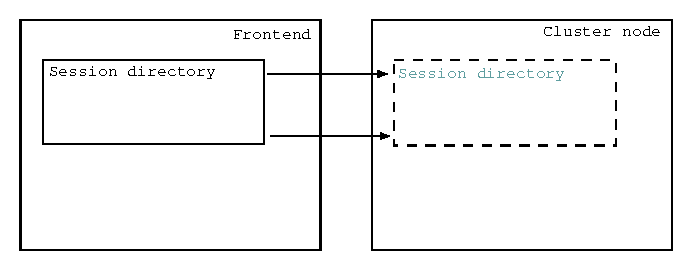
\includegraphics{pic2}
\par\end{centering}


\caption{\label{fig:no node scratch}Both RUNTIME\_LOCAL\_SCRATCH\_DIR and
RUNTIME\_FRONTEND\_SEES\_NODE undefined. Job is executed in session
directory placed on frontend.}
\end{figure}
%
\begin{figure}[htbp]
\begin{centering}
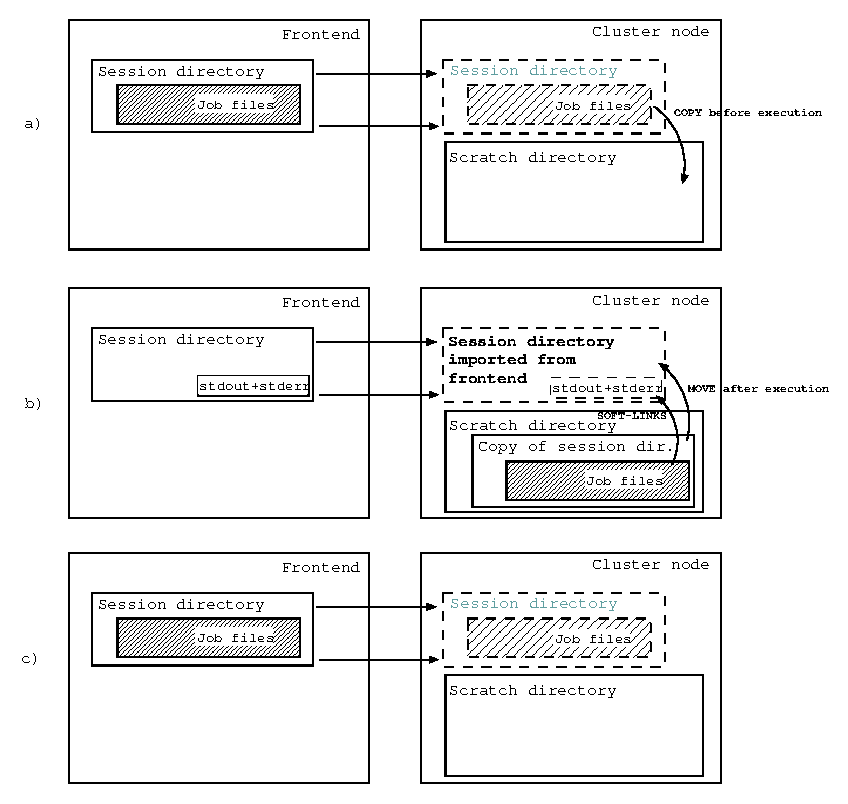
\includegraphics{pic3}
\par\end{centering}


\caption{\label{fig:node scratch, not vis on front}RUNTIME\_LOCAL\_SCRATCH\_DIR
is set to value representing sratch directory on computing node, RUNTIME\_FRONTEND\_SEES\_NODE
undefined.}

\begin{lyxlist}{00.00.0000}
\item [{a)}] After job script starts all input files are moved to 'scratch
directory' on computing node.
\item [{b)}] Job runs in separate directory in 'scratch directory'. Only
files representing job's \textit{stdout} and \textit{stderr} are placed
in original 'session directory' and soft-linked in 'scratch'. After
execution all files from 'scratch' are moved back to original 'session
directory'.
\item [{c)}] All output files are in 'session directory' and are ready
to be uploaded/downloaded.
\end{lyxlist}

\end{figure}
%
\begin{figure}[htbp]
\begin{centering}
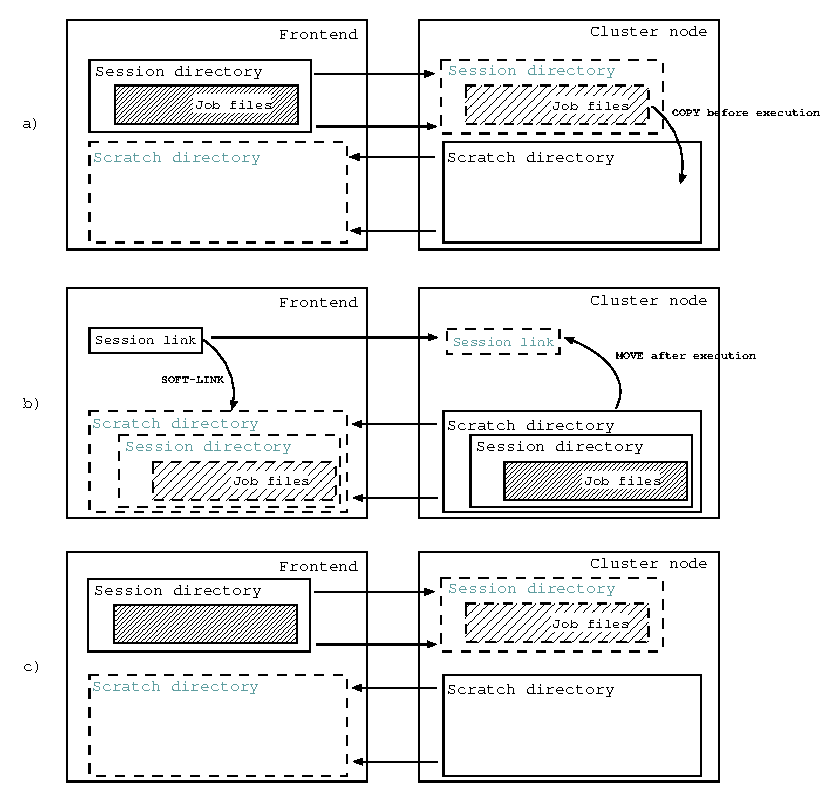
\includegraphics{pic4}
\par\end{centering}


\caption{\label{fig:node scratch, vis on front}Both RUNTIME\_LOCAL\_SCRATCH\_DIR
and RUNTIME\_FRONTEND\_SEES\_NODE are set to valuea representing sratch
directory on computing node and way to access that scratch from frontend
correspondingly.}

\begin{lyxlist}{00.00.0000}
\item [{a)}] After job script starts all input files are moved to 'scratch
directory' on computing node. Original 'session directory' is removed
and replaced with soft-link to copy of session directory in 'scratch'
as seen on frontend.
\item [{b)}] Job runs in separate directory in 'scratch directory'. All
files are also available on frontend through soft-link. After execution
soft-link is replaced with directory and all files from 'scratch'
are moved back to original 'session directory'.
\item [{c)}] All output files are in 'session directory' and are ready
to be uploaded/downloaded. 
\end{lyxlist}

\end{figure}



\subsection{Runtime environment}

The GM can run specially prepared \emph{BASH} scripts prior creation
of job's script, before and after executing job's main executable.
Those scripts are requested by user through \emph{runtimeenvironment}
attribute in RSL and are run with only argument set equal to '0',
'1' or '2' during creation of job's script, before execution of main
executable and after main executable finished accordingly. They all
are run through BASH's 'source' command, and hence can manipulate
with shell variables. With argument '0' scripts are run by the GM
on frontend. Some environment variables are defined in that case and
can be changed to influence job's execution later:

\begin{itemize}
\item joboption\_directory - session directory.
\item joboption\_args - command to be executed as specified in RSL.
\item joboption\_env\_\# - array of 'NAME=VALUE' environment variables (\textbf{not}
bash array).
\item joboption\_runtime\_\# - array of requested \emph{runtimeenvironment}
names (\textbf{not} bash array).
\item joboption\_num - \emph{runtimeenvironment} currently beeing processed
(number starting from 0).
\item joboption\_stdin - name of file to be attached to stdin handle.
\item joboption\_stdout - same for stdout.
\item joboption\_stderr - same for stderr.
\item joboption\_maxcputime - amout of CPU time requested (minutes).
\item joboption\_maxmemory - amout of memory requested (megabytes).
\item joboption\_count - number of processors requested.
\item joboption\_lrms - LRMS to be used to run job.
\item joboption\_queue - name of a queue of LRMS to put job into.
\item joboption\_nodeproperty\_\# - array of properties of computing nodes
(LRMS specific, \textbf{not} bash array).
\item joboption\_jobname - name of the job as given by user.
\item joboption\_rsl - whole RSL for very clever submission scripts.
\item joboption\_rsl\_\emph{name} - RSL attributes and values (like joboption\_rsl\_executable=''/bin/echo'')
\end{itemize}
For example \emph{joboption\_args} could be changed to wrap main executable.
Or \emph{joboption\_runtime} could be expanded if current one depends
on others.

With argument '1' scripts are run just before main executable is run.
They are executed on computing node. Such script can prepare environment
for some third-party software package. A current directory in that
case is one which would be used for execution of job. Variable HOME
also points to that directory.

With argument '2' scripts are executed after main executable finished.
Main purpose is to clean possible changes done by scripts run with
'1' (like removing temporary files). Execution of scripts at that
stage also happens on computing node and is not reliable. If the job
is killed by LRMS they most probably won't be executed.


\section{Installation\label{sec:installation}}

To install GM as part of ARC-enabled site please read {}``NorduGrid
ARC server installation instructions'' at \url{http://www.nordugrid.org/documents/ng-server-install.html}.


\subsection{Requirements}

The GM is mostly written using C++. It was tested and should compile
on recent enough \emph{Linux} systems using \emph{gcc} compiler and
\emph{GNU make} (gcc versions 2.95, 2.96, 3.2, 3.4 were tested). You
will also need \emph{Globus Toolkit$^{TM}$} of version higher than
2.2 \emph{}installed \url{http://www-unix.globus.org/toolkit/}.


\subsection{Setup of the Grid Manager}

For in-depth information about how to properly setup the GM and related
software please read {}``NorduGrid ARC server installation instructions''
at \url{http://www.nordugrid.org/documents/ng-server-install.html}.
Follow that manual to install GM, configure and run it. Additional
tips are described here.

The GM is designed to be able to run both as root and as ordinary
user. You can chose the name of the user by using corresponding command
in configuration file. It is better run GM as root if You want to
serve few users.

The GM writes debug information into a file /var/log/grid-manager.log
by default. . Also file /var/log/gm-jobs.log (default path in configuration
template, turned off by default) contains information about all started
and finished jobs, 2 lines per job (1 when job is started and 1 after
it finished). 


\subsection{Setup of the GridFTP Server}

For in-depth information about how to properly setup the GM and related
software please read {}``NorduGrid ARC server installation instructions''
at \url{http://www.nordugrid.org/documents/ng-server-install.html}.
Follow that manual to install GM, configure and run it. Additional
tips are described here.

To make GFS to interoperate with other parts of the ARC only one \emph{jobplugin.so}
needs to be configured. It is advisable to use the template configuration
file. You can leave only part which configures \textit{jobplugin.so}
plugin.


\subsection{Usage}

Refer to the description of the \emph{User Interface} part \cite{ui}
and extensions to RSL \cite{xrsl} for using the GM.


\subsection{Unix accounts}

Bot GM and GFS are designed to be run by \emph{root} UNIX account
and serve multiple local UNIX and global Grid identities. Nevertheless
it is possible to use \emph{non-root} accounts to run those services.
Although this means some functionality loss described below.

There are no implication on running GFS with \emph{gaclplugin} or
\emph{fileplugin} under \emph{non-root} account as long as only Grid
identity of user is used and all served files and directories are
owned by server's account. 

For combination of GM and GFS with \emph{jobplugin} both services
must be run either by same account or one of services must be run
under \emph{root} account. That is needed because services communicate
over local filesystem, hence must have \emph{full} access to same
set of files.

As long as GFS with \emph{jobplugin} is run under non-root account
there is no mapping from Grid identity to local UNIX account taking
place. All alowed Grid users are assigned server's account and are
then processes by GM using same account. Only way to overcome this
limitation is to run one GFS per local account with proper access
control configured.

Because GM has to represent user's local account while communication
with LRMS, it can serve only account it is run under (unless it is
run under \emph{root} account, of course). Like in case of GFS, multiple
instances of GM may be run, one per local account. That solution causes
another implications. The GM looses possibility to share cached files
among serviced users. It is not also possible to control load on a
frontend by limiting number of simultatenuosly running \emph{downloader}
and \emph{uploader} modules.

One has also take into account that private part of GSI infrastructure
(private key of a host at least) has to be duplicated for every account
used to run GFS.


\section*{Appendix A. Job control over jobplugin.so}


\subsection*{Virtual tree}

Under mount point of jobplugin gridftp client can see directories
representing job belonging to user, who started client. Directory
per job. Directory names are same as jobs' identifiers. Those directories
are directly connected to session directories of jobs and contain
same files and subdirectories. Except if jobs session directory is
moved to computing node. In that case directories only contain files
with redirected stdout and strderr as specified in xRSL.

If job's xRSL has \emph{gmlog} specified job's directory also contains
virtual subdirectory with same name, which contains files with information
about job as created by GM. The most important are 'errors' and 'status'.
'errors' contains stderr of separate modules run by GM in order to
process job (downloader, uploader, job's submission to LRMS). 'status'
contains one word representing state of job. 

Also under mount point there is additional directory named \char`\"{}new\char`\"{}
used to submit new jobs. And another directory {}``info'' with subdirectories
named after job ids. Those subdirectories contain files with information
about job identical to those in subdirectory specified through \emph{gmlog}.


\subsection*{Submission}

Each xRSL put into directory \char`\"{}new\char`\"{} is accepted as
job's description. jobplugin parses it and client gets positive response
if there are no errors in request.

Job gets identifier and directory with corresponding name appears.
If job's description contains input files which should be delivered
from client's machine, client must upload them to that directory under
specified names.

Because each job gets identifier there should be a way for client
to obtain it. For that prior to providing xRSL client sends command
CWD to change current directory to \char`\"{}new\char`\"{}. In this
way job's identifier is reserved, new directory corresponding to that
identifier is created and client is redirected to it (as specified
in FTP protocol). Job's description put into \char`\"{}new\char`\"{}
will get reserved identifier.


\subsection*{Actions}

Various actions to affect processing of existing job are performed
by uploading xRSL files into directory {}``new''. Content of xRSL
may consist of only 2 parameters - action for \emph{action} to be
performed, and \emph{jobid} to identify job to be affected. Rest of
parameters are ignored.

Currently supported actions are:

\begin{lyxlist}{00.00.0000}
\item [{\emph{cancel}}] to cancel job
\item [{\emph{clean}}] to remove job from computing resource
\item [{\emph{renew}}] to renew credentials delegated to job
\item [{\emph{restart}}] to restart job after failure at some phases
\end{lyxlist}
It is also possible to perform some actions by using shortcut FTP
operations described below.


\subsubsection*{Cancel}

Job is canceled by performing DELE (delete file) command on directory
representing job. It can take some time (few minutes) before job is
actually canceled. Nevertheless client gets response immediately.


\subsubsection*{Clean}

Job's content is cleaned by performing RMD (remove directory) command
on directory representing job. If job is in \char`\"{}FINISHED\char`\"{}
state it will be cleaned immediately. Otherwise it will be cleaned
after it reaches state \char`\"{}FINISHED\char`\"{}.


\subsubsection*{Renew}

If client requests CWD to session directory credentials passed during
authentication are compared to current credentials of the job. If
validity time of the new credentials is longer job's credentials are
replaced with new.


\section*{Appendix B. Library \textit{libarcdata}}

\emph{libarcdata} is now part of \emph{libngui} library. It's functions
are declared in a header file \emph{arcdata.h}. They correspond to
ng{*} utilities meant for data handling - \emph{arcacl}, \emph{arccp},
\emph{arcls}, \emph{arcrm}, \emph{arctransfer}. It consists of following
functions:

\begin{lyxcode}
void~arcacl(const~std::string\&~file\_url,~const~std::string\&~command,~int~timeout~=~0);



void~arcregister~(const~std::string\&~source\_url,~const~std::string\&~destination\_url,~bool~secure~=~false,~bool~passive~=~true,~bool~force\_meta~=~false,~int~timeout~=~0);



void~arccp~(const~std::string\&~source\_url,~const~std::string\&~destination\_url,~bool~secure~=~false,~bool~passive~=~true,~bool~force\_meta~=~false,~int~recursion~=~0,~bool~verbose~=~false,~int~timeout~=~0);



void~arcls(const~std::string\&~dir\_url,~bool~show\_details~=~false,~bool~show\_urls~=~false,~int~recursion~=~0,~int~timeout~=~0);



void~arcrm(const~std::string\&~file\_url,~bool~errcont~=~false,~int~timeout~=~0);



void~arctransfer(const~std::string\&~destination,~std::list<std::string>\&~sources,~int~timeout~=~0);
\end{lyxcode}
Additionally this library contains C++ classes used by \emph{ng{*}}
data management utilities. Those are described in {}``ARC::DataMove
Reference Manual''.


\section*{Appendix C. Error messages of GM}

If job has not finished successfully the GM put one or more lines
into \textit{job.ID.failed}. Possible valuesinclude those generated
by the GM itself:

\begin{tabular}{|p{2.5in}|p{4in}|}
\hline 
\emph{Error string}&
\emph{Reason/description}\tabularnewline
\hline 
Internal error&
Error in internal algorithm\tabularnewline
\hline 
Internal error: can't read local file&
Error manipulating files in the control directory\tabularnewline
\hline 
Failed reading local job information&
-//-\tabularnewline
\hline 
Failed reading status of the job&
-//-\tabularnewline
\hline 
Failed writing job status&
-//-\tabularnewline
\hline 
Failed during processing failure&
-//-\tabularnewline
\hline 
Serious troubles (problems during processing problems)&
-//-\tabularnewline
\hline 
Failed initiating job submission to LRMS&
Could not run backend executable to pass job to LRMS\tabularnewline
\hline 
Job submission to LRMS failed&
Backend executable supposed to pass job to LRMs returned non-zero
exit code\tabularnewline
\hline 
Failed extracting LRMS ID due to some internal error&
Output of Backend executable supposed to contain local ID of passed
job could not be parsed\tabularnewline
\hline 
Failed in files upload (post-processing)&
Failed to upload some or all output files\tabularnewline
\hline 
Failed in files upload due to expired credentials - try to renew&
Failed to upload some or all output files most probably due to expired
credentials (proxy certificate)\tabularnewline
\hline 
Failed to run uploader (post-processing)&
Could not run \emph{uploader} executable\tabularnewline
\hline 
uploader failed (postprocessing)&
Generic error related to \emph{uploader} component\tabularnewline
\hline 
Failed in files download (pre-processing)&
Failed to upload some or all input files\tabularnewline
\hline 
Failed in files download due to expired credentials - try to renew&
Failed to download some or all input files most probably due to expired
credentials (proxy certificate)\tabularnewline
\hline 
Failed to run downloader (pre-processing)&
Could not run \emph{downloader} executable\tabularnewline
\hline
downloader failed (preprocessing)&
Generic error related to \emph{downloader} component\tabularnewline
\hline
User requested to cancel the job&
GM detected external request to cancel this job, most probably issued
by user\tabularnewline
\hline
Could not process RSL&
Job description could not be processed to syntax errors or missing
elements\tabularnewline
\hline
User requested dryrun. Job skiped.&
Job description contains request not to process this job\tabularnewline
\hline
LRMS error: (CODE) DESCRIPTION&
LRMS returned error. CODE is replaced with numeric code of LRMS, and
DESCRIPTION with textual description\tabularnewline
\hline
Plugin at state STATE failed: OUTPUT&
External plugin specified in GM's configuration returned non-zero
exit code. STATE is replcaced by name of state to which job was going
to be passed, OUTPUT by textual output generated by plugin.\tabularnewline
\hline
Failed running plugin at state STATE&
External plugin specified in GM's configuration could not be executed.\tabularnewline
\hline
\end{tabular}

\medskip{}
Provided by downloader component (URL is replcaced by source of input
file, FILE by name of file):

\begin{tabular}{|p{2.5in}|p{4in}|}
\hline 
\emph{Error string}&
\emph{Reason/description}\tabularnewline
\hline 
Internal error in downloader&
Generic error \tabularnewline
\hline 
Input file: URL - unknown error&
Generic error \tabularnewline
\hline 
Input file: URL - unexpected error&
Generic error \tabularnewline
\hline 
Input file: URL - bad source URL&
Source URL is either malformed or not supported\tabularnewline
\hline 
Input file: URL - bad destination URL&
Shouldn't happen\tabularnewline
\hline 
Input file: URL - failed to resolve source locations&
File either not registred or other problems related to Data Indexing
service.\tabularnewline
\hline 
Input file: URL - failed to resolve destination locations&
Shouldn't happen\tabularnewline
\hline 
Input file: URL - failed to register new destination file&
Shouldn't happen\tabularnewline
\hline 
Input file: URL - can't start reading from source&
Problems related to accessing instance of file at Data Storing service.\tabularnewline
\hline 
Input file: URL - can't read from source&
-//-\tabularnewline
\hline 
Input file: URL - can't start writing to destination&
Access problems in a session directory\tabularnewline
\hline 
Input file: URL - can't write to destination&
-//-\tabularnewline
\hline 
Input file: URL - data transfer was too slow&
Timeouted while trying to download file\tabularnewline
\hline 
Input file: URL - failed while closing connection to source&
Shouldn't happen\tabularnewline
\hline 
Input file: URL - failed while closing connection to destination&
Shouldn't happen\tabularnewline
\hline 
Input file: URL - failed to register new location&
Shouldn't happen\tabularnewline
\hline 
Input file: URL - can't use local cache&
Problems with GM cache \tabularnewline
\hline 
Input file: URL - system error&
Operating System returned error code where unexpected\tabularnewline
\hline 
Input file: URL - delegated credentials expired&
Access to source requires credententials and they are either outdated
or missing (not delegated).\tabularnewline
\hline 
User file: FILENAME - Bad information about file: checksum can't be
parsed.&
In job description there is a checksum provided for file uploadable
by user interface and this record can't be interpreted.\tabularnewline
\hline 
User file: FILENAME - Bad information about file: size can't be parsed.&
In job description there is a size provided for file uploadable by
user interface and this record can't be interpreted.\tabularnewline
\hline 
User file: FILENAME - Expected file. Directory found.&
Instead of file uploadable by user interface GM found directory with
same name in a session directory.\tabularnewline
\hline 
User file: FILENAME - Expected ordinary file. Special object found.&
Instead of file uploadable by user interface GM found special object
with same name in a session directory.\tabularnewline
\hline 
User file: FILENAME - Delivered file is bigger than specified.&
The size of file uploadable by user interface is bigger than specified
in job description.\tabularnewline
\hline
User file: FILENAME - Delivered file is unreadable.&
GM can't check user uploadable file due to some internal error. Most
probably due to improperly configured local permissions.\tabularnewline
\hline
User file: FILENAME - Could not read file to compute checksum.&
GM can't read user uploadable file due to some internal error. Most
probably due to improperly configured local permissions.\tabularnewline
\hline
User file: FILENAME - Timeout waiting&
GM waited for user uploadable file too long.\tabularnewline
\hline
\end{tabular}

\medskip{}
Provided by uploader component (URL is replcaced by destination of
output file) :

\begin{tabular}{|p{2.5in}|p{4in}|}
\hline 
\emph{Error string}&
\emph{Reason/description}\tabularnewline
\hline 
Internal error in uploader&
Generic error \tabularnewline
\hline 
Output file: URL - unknown error&
Generic error \tabularnewline
\hline 
Output file: URL - unexpected error&
Generic error \tabularnewline
\hline 
User requested to store output locally URL&
Destination is URL of type \emph{file}.\tabularnewline
\hline 
Output file: URL - bad source URL&
Shouldn't happen\tabularnewline
\hline 
Output file: URL - bad destination URL&
Destination URL is either malformed or not supported\tabularnewline
\hline 
Output file: URL - failed to resolve source locations&
Shouldn't happen\tabularnewline
\hline 
Output file: URL - failed to resolve destination locations&
Problems related to Data Indexing service.\tabularnewline
\hline 
Output file: URL - failed to register new destination file&
-//-\tabularnewline
\hline 
Output file: URL - can't start reading from source&
User request to store output file, but there is no such file or there
are problems accessing session directory\tabularnewline
\hline 
Output file: URL - can't start writing to destination&
Problems with Data Storing services\tabularnewline
\hline 
Output file: URL - can't read from source&
Problems accessing session directory\tabularnewline
\hline 
Output file: URL - can't write to destination&
Problems with Data Storing services\tabularnewline
\hline 
Output file: URL - data transfer was too slow&
Timeout during transfer\tabularnewline
\hline 
Output file: URL - failed while closing connection to source&
Shouldn't happen\tabularnewline
\hline 
Output file: URL - failed while closing connection to destination&
Shouldn't happen\tabularnewline
\hline 
Output file: URL - failed to register new location&
Problems related to Data Indexing service.\tabularnewline
\hline 
Output file: URL - can't use local cache&
Shouldn't happen\tabularnewline
\hline 
Output file: URL - system error&
Operating System returned error code where unexpected\tabularnewline
\hline 
Output file: URL - delegated credentials expired&
Access to destination requires credententials and they are either
outdated or missing (not delegated).\tabularnewline
\hline 
&
\tabularnewline
\hline
&
\tabularnewline
\hline
\end{tabular}

\medskip{}
Coming from LRMS (PBS) backend:

\begin{tabular}{|p{2.5in}|p{4in}|}
\hline 
\emph{Error string}&
\emph{Reason/description}\tabularnewline
\hline 
Submission: Configuration error.&
\tabularnewline
\hline 
Submission: System error.&
\tabularnewline
\hline 
Submission: Job description error.&
\tabularnewline
\hline 
Submission: Local submission client behaved unexpectedly.&
\tabularnewline
\hline 
Submission: Local submission client failed.&
\tabularnewline
\hline
\end{tabular}

\begin{lyxcode}
~
\end{lyxcode}

\section*{Appendix D. A-Rex WSDL}

\begin{lyxcode}
<?xml~version=\char`\"{}1.0\char`\"{}~encoding=\char`\"{}UTF-8\char`\"{}?>

<wsdl:definitions~targetNamespace=\char`\"{}http://www.nordugrid.org/schemas/a-rex\char`\"{}

~xmlns:SOAP-ENV=\char`\"{}http://schemas.xmlsoap.org/soap/envelope/\char`\"{}

~xmlns:SOAP-ENC=\char`\"{}http://schemas.xmlsoap.org/soap/encoding/\char`\"{}

~xmlns:xsi=\char`\"{}http://www.w3.org/2001/XMLSchema-instance\char`\"{}

~xmlns:xsd=\char`\"{}http://www.w3.org/2001/XMLSchema\char`\"{}

~xmlns:soap=\char`\"{}http://schemas.xmlsoap.org/wsdl/soap/\char`\"{}

~xmlns:wsdl=\char`\"{}http://schemas.xmlsoap.org/wsdl/\char`\"{}

~xmlns:wsa=\char`\"{}http://www.w3.org/2005/08/addressing\char`\"{}

~xmlns:bes-factory=\char`\"{}http://schemas.ggf.org/bes/2006/08/bes-factory\char`\"{}

~xmlns:bes-mgmt=\char`\"{}http://schemas.ggf.org/bes/2006/08/bes-management\char`\"{}

~xmlns:deleg=\char`\"{}http://www.nordugrid.org/schemas/delegation\char`\"{}

~xmlns:wsrf-rpw=\char`\"{}http://docs.oasis-open.org/wsrf/rpw-2\char`\"{}

~xmlns:a-rex=\char`\"{}http://www.nordugrid.org/schemas/a-rex\char`\"{}>

~~<wsdl:import~namespase=\char`\"{}http://schemas.ggf.org/bes/2006/08/bes-factory\char`\"{}~location=\char`\"{}./bes-factory.wsdl\char`\"{}/>

~~<wsdl:import~namespase=\char`\"{}http://schemas.ggf.org/bes/2006/08/bes-management\char`\"{}~location=\char`\"{}./bes-management.wsdl\char`\"{}/>

~~<wsdl:import~namespase=\char`\"{}http://www.nordugrid.org/schemas/delegation\char`\"{}~location=\char`\"{}../schemas/delegation.wsdl\char`\"{}/>

~~<wsdl:import~namespase=\char`\"{}http://docs.oasis-open.org/wsrf/rpw-2\char`\"{}~location=\char`\"{}http://docs.oasis-open.org/wsrf/rpw-2.wsdl\char`\"{}/>

~~<wsdl:types>

~~~~<xsd:schema~targetNamespace=\char`\"{}http://www.nordugrid.org/schemas/a-rex\char`\"{}>

~~~~~~<xsd:import~namespace=\char`\"{}http://www.w3.org/2005/08/addressing\char`\"{}~schemaLocation=\char`\"{}./ws-addr.xsd\char`\"{}/>

~~~~~~<xsd:simpleType~name=\char`\"{}ActivitySubStateType\char`\"{}>

~~~~~~~~<xsd:restriction~base=\char`\"{}xsd:string\char`\"{}>

~~~~~~~~~~<xsd:enumeration~value=\char`\"{}Accepting\char`\"{}/>

~~~~~~~~~~<xsd:enumeration~value=\char`\"{}Accepted\char`\"{}/>

~~~~~~~~~~<xsd:enumeration~value=\char`\"{}Preparing\char`\"{}/>

~~~~~~~~~~<xsd:enumeration~value=\char`\"{}Prepared\char`\"{}/>

~~~~~~~~~~<xsd:enumeration~value=\char`\"{}Submiting\char`\"{}/>

~~~~~~~~~~<xsd:enumeration~value=\char`\"{}Executing\char`\"{}/>

~~~~~~~~~~<xsd:enumeration~value=\char`\"{}Killing\char`\"{}/>

~~~~~~~~~~<xsd:enumeration~value=\char`\"{}Executed\char`\"{}/>

~~~~~~~~~~<xsd:enumeration~value=\char`\"{}Finishing\char`\"{}/>

~~~~~~~~~~<xsd:enumeration~value=\char`\"{}Finished\char`\"{}/>

~~~~~~~~~~<xsd:enumeration~value=\char`\"{}Failed\char`\"{}/>

~~~~~~~~~~<xsd:enumeration~value=\char`\"{}Deleted\char`\"{}/>

~~~~~~~~~~<xsd:enumeration~value=\char`\"{}Pending\char`\"{}/>

~~~~~~~~~~<xsd:enumeration~value=\char`\"{}Held\char`\"{}/>

~~~~~~~~</xsd:restriction>

~~~~~~</xsd:simpleType>

~~~~~~<xsd:element~name=\char`\"{}State\char`\"{}~type=\char`\"{}a-rex:ActivitySubStateType\char`\"{}/>

~~~~~~<xsd:complexType~name=\char`\"{}ResourceInformationDocumentType\char`\"{}>

~~~~~~~~<xsd:sequence>

~~~~~~~~~~~<xsd:element~name=\char`\"{}BESFactory\char`\"{}~type=\char`\"{}bes-factory:FactoryResourceAttributesDocumentType\char`\"{}/>

~~~~~~~~~~<xsd:complexType~name=\char`\"{}Glue2Resource\char`\"{}~minOccurs='0'>

~~~~~~~~~~~~<xsd:sequence>

~~~~~~~~~~~~~~<xsd:any~namespace=\char`\"{}\#\#other\char`\"{}~processContents=\char`\"{}lax\char`\"{}~minOccurs=\char`\"{}0\char`\"{}~maxOccurs=\char`\"{}unbounded\char`\"{}/>

~~~~~~~~~~~~</xsd:sequence>

~~~~~~~~~~</xsd:complexType>

~~~~~~~~~~<xsd:complexType~name=\char`\"{}Activities\char`\"{}~minOccurs='0'>

~~~~~~~~~~~~<xsd:sequence>

~~~~~~~~~~~~~~<xsd:complexType~name=\char`\"{}Activity\char`\"{}~minOccurs='0'~maxOccurs='unbounded'>

~~~~~~~~~~~~~~~~<xsd:sequence>

~~~~~~~~~~~~~~~~~~<xsd:element~name=\char`\"{}ActivityIdentifier\char`\"{}~type=\char`\"{}wsa:EndpointReferenceType\char`\"{}/>

~~~~~~~~~~~~~~~~~~<xsd:element~ref=\char`\"{}bes-factory:ActivityDocument\char`\"{}~minOccurs='0'/>

~~~~~~~~~~~~~~~~~~<xsd:complexType~name=\char`\"{}Glue2Job\char`\"{}~minOccurs='0'>

~~~~~~~~~~~~~~~~~~~~<xsd:sequence>

~~~~~~~~~~~~~~~~~~~~~~<xsd:any~namespace=\char`\"{}\#\#other\char`\"{}~processContents=\char`\"{}lax\char`\"{}~minOccurs=\char`\"{}0\char`\"{}~maxOccurs=\char`\"{}unbounded\char`\"{}/>

~~~~~~~~~~~~~~~~~~~~</xsd:sequence>

~~~~~~~~~~~~~~~~~~</xsd:complexType>

~~~~~~~~~~~~~~~~</xsd:sequence>

~~~~~~~~~~~~~~</xsd:complexType>

~~~~~~~~~~~~</xsd:sequence>

~~~~~~~~~~</xsd:complexType>

~~~~~~~~</xsd:sequence>

~~~~~~</xsd:complexType>

~~~~~~<xsd:complexType~name=\char`\"{}ChangeActivityStatusRequestType\char`\"{}>

~~~~~~~~<xsd:sequence>

~~~~~~~~~~<xsd:element~name=\char`\"{}ActivityIdentifier\char`\"{}~type=\char`\"{}wsa:EndpointReferenceType\char`\"{}/>

~~~~~~~~~~<xsd:element~name=\char`\"{}OldStatus\char`\"{}~type=\char`\"{}bes-factory:ActivityStatusType\char`\"{}~minOccurs=\char`\"{}0\char`\"{}/>

~~~~~~~~~~<xsd:element~name=\char`\"{}NewStatus\char`\"{}~type=\char`\"{}bes-factory:ActivityStatusType\char`\"{}/>

~~~~~~~~</xsd:sequence>

~~~~~~</xsd:complexType>

~~~~~~<xsd:element~name=\char`\"{}ChangeActivityStatus\char`\"{}~type=\char`\"{}a-rex:ChangeActivityStatusRequestType\char`\"{}/>

~~~~~~<xsd:complexType~name=\char`\"{}ChangeActivityStatusResponseType\char`\"{}>

~~~~~~~~<xsd:sequence>

~~~~~~~~~~<xsd:element~name=\char`\"{}NewStatus\char`\"{}~type=\char`\"{}bes-factory:ActivityStatusType\char`\"{}/>

~~~~~~~~</xsd:sequence>

~~~~~~</xsd:complexType>

~~~~~~<xsd:element~name=\char`\"{}ChangeActivityStatusResponse\char`\"{}~type=\char`\"{}a-rex:ChangeActivityStatusResponseType\char`\"{}/>

~~~~</xsd:schema>

~~</wsdl:types>

~~<wsdl:message~name=\char`\"{}ChangeActivityStatusRequest\char`\"{}>

~~~~<wsdl:part~name=\char`\"{}ChangeActivityStatusRequest\char`\"{}~element=\char`\"{}a-rex:ChangeActivityStatus\char`\"{}/>

~~</wsdl:message>

~~<wsdl:message~name=\char`\"{}ChangeActivityStatusResponse\char`\"{}>

~~~~<wsdl:part~name=\char`\"{}ChangeActivityStatusResponse\char`\"{}~element=\char`\"{}a-rex:ChangeActivityStatusResponse\char`\"{}/>

~~</wsdl:message>

~~<wsdl:portType~name=\char`\"{}a-rex\char`\"{}>

~~~~<wsdl:operation~name=\char`\"{}ChangeActivityStatus\char`\"{}>

~~~~~~<wsdl:documentation>

~~~~~~~~This~operation~allows~any~simple~status~change~request

~~~~~~~~which~involves~no~additional~parameters.~It~should~be

~~~~~~~~used~to~modify~job/activity~execution~flow:

~~~~~~~~~~-~To~put~job~on~hold

~~~~~~~~~~-~To~rerun~job~in~case~of~failure

~~~~~~~~~~-~To~cancel~job~(same~as~TerminateActivity~of~BESFActory)

~~~~~~~~~~-~To~remove/release~job~-~as~long~as~non-existence~is~a~state

~~~~~~~~~~-~Any~other~status~change~no~supported~by~BES

~~~~~~</wsdl:documentation>

~~~~~~<wsdl:input~name=\char`\"{}ChangeActivityStatusRequest\char`\"{}

~~~~~~~~message=\char`\"{}a-rex:ChangeActivityStatusRequest\char`\"{}/>

~~~~~~<wsdl:output~name=\char`\"{}ChangeActivityStatusResponse\char`\"{}

~~~~~~~~message=\char`\"{}a-rex:ChangeActivityStatusResponse\char`\"{}/>

~~~~~~<wsdl:fault~name=\char`\"{}NotAuthorizedFault\char`\"{}

~~~~~~~~message=\char`\"{}bes-factory:NotAuthorizedFault\char`\"{}

~~~~~~~~wsa:Action=\char`\"{}http://schemas.ggf.org/bes/2006/08/bes-factory/BESFactoryPortType/Fault\char`\"{}/>

~~~~~~<wsdl:fault~name=\char`\"{}InvalidActivityIdentifierFault\char`\"{}

~~~~~~~~message=\char`\"{}bes-factory:InvalidActivityIdentifierFault\char`\"{}

~~~~~~~~wsa:Action=\char`\"{}http://schemas.ggf.org/bes/2006/08/bes-factory/BESFactoryPortType/Fault\char`\"{}/>

~~~~~~<wsdl:fault~name=\char`\"{}CantApplyOperationToCurrentStateFault\char`\"{}

~~~~~~~~~message=\char`\"{}bes-factory:CantApplyOperationToCurrentStateFault\char`\"{}

~~~~~~~~~wsa:Action=\char`\"{}http://schemas.ggf.org/bes/2006/08/bes-factory/BESFactoryPortType/Fault\char`\"{}/>

~~~~~~<wsdl:fault~name=\char`\"{}OperationWillBeAppliedEventuallyFault\char`\"{}

~~~~~~~~~message=\char`\"{}bes-factory:OperationWillBeAppliedEventuallyFault\char`\"{}

~~~~~~~~~wsa:Action=\char`\"{}http://schemas.ggf.org/bes/2006/08/bes-factory/BESFactoryPortType/Fault\char`\"{}/>

~~~~</wsdl:operation>

~~</wsdl:portType>

~~<wsdl:binding~name=\char`\"{}a-rex\char`\"{}~type=\char`\"{}a-rex:a-rex\char`\"{}>

~~~~<soap:binding~style=\char`\"{}document\char`\"{}~transport=\char`\"{}http://schemas.xmlsoap.org/soap/http\char`\"{}/>

~~~~<wsdl:operation~name=\char`\"{}ChangeActivityStatus\char`\"{}>

~~~~~~<soap:operation~soapAction=\char`\"{}ChangeActivityStatus\char`\"{}/>

~~~~~~<wsdl:input~name=\char`\"{}ChangeActivityStatusRequest\char`\"{}>

~~~~~~~~~<soap:body~use=\char`\"{}literal\char`\"{}/>

~~~~~~</wsdl:input>

~~~~~~<wsdl:output~name=\char`\"{}ChangeActivityStatusResponse\char`\"{}>

~~~~~~~~~<soap:body~use=\char`\"{}literal\char`\"{}/>

~~~~~~</wsdl:output>

~~~~~~<wsdl:fault~name=\char`\"{}NotAuthorizedFault\char`\"{}>

~~~~~~~~<soap:fault~name=\char`\"{}NotAuthorizedFault\char`\"{}~use=\char`\"{}literal\char`\"{}~/>

~~~~~~</wsdl:fault>

~~~~~~<wsdl:fault~name=\char`\"{}InvalidActivityIdentifierFault\char`\"{}>

~~~~~~~~<soap:fault~name=\char`\"{}InvalidActivityIdentifierFault\char`\"{}~use=\char`\"{}literal\char`\"{}~/>

~~~~~~</wsdl:fault>

~~~~~~<wsdl:fault~name=\char`\"{}CantApplyOperationToCurrentStateFault\char`\"{}>

~~~~~~~~<soap:fault~name=\char`\"{}CantApplyOperationToCurrentStateFault\char`\"{}~use=\char`\"{}literal\char`\"{}~/>

~~~~~~</wsdl:fault>

~~~~~~<wsdl:fault~name=\char`\"{}OperationWillBeAppliedEventuallyFault\char`\"{}>

~~~~~~~~<soap:fault~name=\char`\"{}OperationWillBeAppliedEventuallyFault\char`\"{}~use=\char`\"{}literal\char`\"{}~/>

~~~~~~</wsdl:fault>

~~~~</wsdl:operation>

~~</wsdl:binding>

~~<wsdl:binding~name=\char`\"{}GetResourcePropertyDocument\char`\"{}~type=\char`\"{}wsrf-rpw:GetResourcePropertyDocument\char`\"{}>

~~~~<soap:binding~style=\char`\"{}document\char`\"{}~transport=\char`\"{}http://schemas.xmlsoap.org/soap/http\char`\"{}/>

~~~~<wsdl:operation~name=\char`\"{}GetResourcePropertyDocument\char`\"{}>

~~~~~~<soap:operation~soapAction=\char`\"{}GetResourcePropertyDocument\char`\"{}/>

~~~~~~<wsdl:input~name=\char`\"{}wsrf-rpw:GetResourcePropertyDocumentRequest\char`\"{}>

~~~~~~~~<soap:body~use=\char`\"{}literal\char`\"{}/>

~~~~~~</wsdl:input>

~~~~~~<wsdl:output~name=\char`\"{}wsrf-rpw:GetResourcePropertyDocumentResponse\char`\"{}>

~~~~~~~~<soap:body~use=\char`\"{}literal\char`\"{}/>

~~~~~~</wsdl:output>

~~~~~~<wsdl:fault~name=\char`\"{}ResourceUnknownFault\char`\"{}>

~~~~~~~~<soap:fault~name=\char`\"{}ResourceUnknownFault\char`\"{}~use=\char`\"{}literal\char`\"{}~/>

~~~~~~</wsdl:fault>

~~~~~~<wsdl:fault~name=\char`\"{}ResourceUnavailableFault\char`\"{}>

~~~~~~~~<soap:fault~name=\char`\"{}ResourceUnavailabbleFault\char`\"{}~use=\char`\"{}literal\char`\"{}~/>

~~~~~~</wsdl:fault>

~~~~</wsdl:operation>

~~</wsdl:binding>

~~<wsdl:binding~name=\char`\"{}GetResourceProperty\char`\"{}~type=\char`\"{}wsrf-rpw:GetResourceProperty\char`\"{}>

~~~~<soap:binding~style=\char`\"{}document\char`\"{}~transport=\char`\"{}http://schemas.xmlsoap.org/soap/http\char`\"{}/>

~~~~<wsdl:operation~name=\char`\"{}GetResourceProperty\char`\"{}>

~~~~~~<soap:operation~soapAction=\char`\"{}GetResourceProperty\char`\"{}/>

~~~~~~<wsdl:input~name=\char`\"{}wsrf-rpw:GetResourcePropertyRequest\char`\"{}>

~~~~~~~~<soap:body~use=\char`\"{}literal\char`\"{}/>

~~~~~~</wsdl:input>

~~~~~~<wsdl:output~name=\char`\"{}wsrf-rpw:GetResourcePropertyResponse\char`\"{}>

~~~~~~~~<soap:body~use=\char`\"{}literal\char`\"{}/>

~~~~~~</wsdl:output>

~~~~~~<wsdl:fault~name=\char`\"{}ResourceUnknownFault\char`\"{}>

~~~~~~~~<soap:fault~name=\char`\"{}ResourceUnknownFault\char`\"{}~use=\char`\"{}literal\char`\"{}~/>

~~~~~~</wsdl:fault>

~~~~~~<wsdl:fault~name=\char`\"{}ResourceUnavailableFault\char`\"{}>

~~~~~~~~<soap:fault~name=\char`\"{}ResourceUnavailabbleFault\char`\"{}~use=\char`\"{}literal\char`\"{}~/>

~~~~~~</wsdl:fault>

~~~~~~<wsdl:fault~name=\char`\"{}InvalidResourcePropertyQNameFault\char`\"{}>

~~~~~~~~<soap:fault~name=\char`\"{}InvalidResourcePropertyQNameFault\char`\"{}~use=\char`\"{}literal\char`\"{}~/>

~~~~~~</wsdl:fault>

~~~~</wsdl:operation>

~~</wsdl:binding>

~~<wsdl:binding~name=\char`\"{}QueryResourceProperties\char`\"{}~type=\char`\"{}wsrf:QueryResourceProperties\char`\"{}>

~~~~<soap:binding~style=\char`\"{}document\char`\"{}~transport=\char`\"{}http://schemas.xmlsoap.org/soap/http\char`\"{}/>

~~~~<wsdl:operation~name=\char`\"{}QueryResourceProperties\char`\"{}>

~~~~~~<soap:operation~soapAction=\char`\"{}QueryResourceProperties\char`\"{}/>

~~~~~~<wsdl:input~name=\char`\"{}wsrf-rpw:QueryResourcePropertiesRequest\char`\"{}>

~~~~~~~~<soap:body~use=\char`\"{}literal\char`\"{}/>

~~~~~~</wsdl:input>

~~~~~~<wsdl:output~name=\char`\"{}wsrf-rpw:QueryResourcePropertiesResponse\char`\"{}>

~~~~~~~~<soap:body~use=\char`\"{}literal\char`\"{}/>

~~~~~~</wsdl:output>

~~~~~~<wsdl:fault~name=\char`\"{}ResourceUnknownFault\char`\"{}>

~~~~~~~~<soap:fault~name=\char`\"{}ResourceUnknownFault\char`\"{}~use=\char`\"{}literal\char`\"{}~/>

~~~~~~</wsdl:fault>

~~~~~~<wsdl:fault~name=\char`\"{}ResourceUnavailableFault\char`\"{}>

~~~~~~~~<soap:fault~name=\char`\"{}ResourceUnavailabbleFault\char`\"{}~use=\char`\"{}literal\char`\"{}~/>

~~~~~~</wsdl:fault>

~~~~~~<wsdl:fault~name=\char`\"{}InvalidResourcePropertyQNameFault\char`\"{}>

~~~~~~~~<soap:fault~name=\char`\"{}InvalidResourcePropertyQNameFault\char`\"{}~use=\char`\"{}literal\char`\"{}~/>

~~~~~~</wsdl:fault>

~~~~~~<wsdl:fault~name=\char`\"{}UnknownQueryExpressionDialectFault\char`\"{}>

~~~~~~~~<soap:fault~name=\char`\"{}UnknownQueryExpressionDialectFault\char`\"{}~use=\char`\"{}literal\char`\"{}~/>

~~~~~~</wsdl:fault>

~~~~~~<wsdl:fault~name=\char`\"{}InvalidQueryExpressionFault\char`\"{}>

~~~~~~~~<soap:fault~name=\char`\"{}InvalidQueryExpressionFault\char`\"{}~use=\char`\"{}literal\char`\"{}~/>

~~~~~~</wsdl:fault>

~~~~~~<wsdl:fault~name=\char`\"{}QueryEvaluationErrorFault\char`\"{}>

~~~~~~~~<soap:fault~name=\char`\"{}QueryEvaluationErrorFault\char`\"{}~use=\char`\"{}literal\char`\"{}~/>

~~~~~~</wsdl:fault>

~~~~</wsdl:operation>

~~</wsdl:binding>

~~<wsdl:service~name=\char`\"{}a-rex\char`\"{}>

~~~~<wsdl:port~name=\char`\"{}delegation\char`\"{}~binding=\char`\"{}deleg:DelegationBinding\char`\"{}>

~~~~</wsdl:port>

~~~~<wsdl:port~name=\char`\"{}bes-factory\char`\"{}~binding=\char`\"{}bes-factory:BESFactoryBinding\char`\"{}>

~~~~</wsdl:port>

~~~~<wsdl:port~name=\char`\"{}bes-mgmt\char`\"{}~binding=\char`\"{}bes-mgmt:BESManagementBinding\char`\"{}>

~~~~</wsdl:port>

~~~~<wsdl:port~name=\char`\"{}GetResourcePropertyDocument\char`\"{}~binding=\char`\"{}a-rex:GetResourcePropertyDocument\char`\"{}>

~~~~</wsdl:port>

~~~~<wsdl:port~name=\char`\"{}GetResourceProperty\char`\"{}~binding=\char`\"{}a-rex:GetResourceProperty\char`\"{}>

~~~~</wsdl:port>

~~~~<wsdl:port~name=\char`\"{}QueryResourceProperties\char`\"{}~binding=\char`\"{}a-rex:QueryResourceProperties\char`\"{}>

~~~~</wsdl:port>

~~~~<wsdl:port~name=\char`\"{}a-rex\char`\"{}~binding=\char`\"{}a-rex:a-rex\char`\"{}>

~~~~</wsdl:port>

~~</wsdl:service>

</wsdl:definitions>
\end{lyxcode}

\section*{Appendix E. Delegation WSDL}

\begin{lyxcode}
<?xml~version=\char`\"{}1.0\char`\"{}~encoding=\char`\"{}UTF-8\char`\"{}?>

<wsdl:definitions~targetNamespace=\char`\"{}http://www.nordugrid.org/schemas/delegation\char`\"{}

~xmlns:SOAP-ENV=\char`\"{}http://schemas.xmlsoap.org/soap/envelope/\char`\"{}

~xmlns:SOAP-ENC=\char`\"{}http://schemas.xmlsoap.org/soap/encoding/\char`\"{}

~xmlns:xsi=\char`\"{}http://www.w3.org/2001/XMLSchema-instance\char`\"{}

~xmlns:xsd=\char`\"{}http://www.w3.org/2001/XMLSchema\char`\"{}

~xmlns:soap=\char`\"{}http://schemas.xmlsoap.org/wsdl/soap/\char`\"{}

~xmlns:wsdl=\char`\"{}http://schemas.xmlsoap.org/wsdl/\char`\"{}

~xmlns:wsa=\char`\"{}http://www.w3.org/2005/08/addressing\char`\"{}

~xmlns:deleg=\char`\"{}http://www.nordugrid.org/schemas/delegation\char`\"{}>

~~<wsdl:types>

~~~~<xsd:schema~targetNamespace=\char`\"{}http://www.nordugrid.org/schemas/delegation\char`\"{}>

~~~~~~<!-{}-~Common~types~-{}->

~~~~~~<xsd:simpleType~name=\char`\"{}TokenFormatType\char`\"{}>

~~~~~~~~<xsd:restriction~base=\char`\"{}xsd:string\char`\"{}>

~~~~~~~~~~<xsd:enumeration~value=\char`\"{}x509\char`\"{}/>

~~~~~~~~</xsd:restriction>

~~~~~~</xsd:simpleType>

~~~~~~<xsd:complexType~name=\char`\"{}ReferenceType\char`\"{}>

~~~~~~~~<xsd:sequence>

~~~~~~~~~~<xsd:any~namespace=\char`\"{}\#\#other\char`\"{}~processContents=\char`\"{}lax\char`\"{}~minOccurs=\char`\"{}0\char`\"{}~maxOccurs=\char`\"{}unbounded\char`\"{}/>

~~~~~~~~</xsd:sequence>

~~~~~~</xsd:complexType>

~~~~~~<xsd:complexType~name=\char`\"{}DelegatedTokenType\char`\"{}>

~~~~~~~~<xsd:sequence>

~~~~~~~~~~<xsd:element~name=\char`\"{}Id\char`\"{}~type=\char`\"{}xsd:string\char`\"{}/>

~~~~~~~~~~<xsd:element~name=\char`\"{}Value\char`\"{}~type=\char`\"{}xsd:string\char`\"{}/>

~~~~~~~~~~<xsd:element~name=\char`\"{}Reference\char`\"{}~type=\char`\"{}deleg:ReferenceType\char`\"{}~minOccurs=\char`\"{}0\char`\"{}~maxOccurs=\char`\"{}unbounded\char`\"{}/>

~~~~~~~~</xsd:sequence>

~~~~~~~~<xsd:attribute~name=\char`\"{}Format\char`\"{}~type=\char`\"{}deleg:TokenFormatType\char`\"{}~use=\char`\"{}required\char`\"{}/>

~~~~~~</xsd:complexType>

~~~~~~<xsd:element~name=\char`\"{}DelegatedToken\char`\"{}~type=\char`\"{}deleg:DelegatedTokenType\char`\"{}/>

~~~~~~<xsd:complexType~name=\char`\"{}TokenRequestType\char`\"{}>

~~~~~~~~<xsd:sequence>

~~~~~~~~~~<xsd:element~name=\char`\"{}Id\char`\"{}~type=\char`\"{}xsd:string\char`\"{}/>

~~~~~~~~~~<xsd:element~name=\char`\"{}Value\char`\"{}~type=\char`\"{}xsd:string\char`\"{}/>

~~~~~~~~</xsd:sequence>

~~~~~~~~<xsd:attribute~name=\char`\"{}Format\char`\"{}~type=\char`\"{}deleg:TokenFormatType\char`\"{}~use=\char`\"{}required\char`\"{}/>

~~~~~~</xsd:complexType>

~~~~~~<xsd:element~name=\char`\"{}TokenRequest\char`\"{}~type=\char`\"{}deleg:TokenRequestType\char`\"{}/>

~~~~~~<!-{}-~Types~for~messages~-{}->

~~~~~~<xsd:complexType~name=\char`\"{}DelegateCredentialsInitRequestType\char`\"{}>

~~~~~~~~<xsd:sequence>

~~~~~~~~</xsd:sequence>

~~~~~~</xsd:complexType>

~~~~~~<xsd:element~name=\char`\"{}DelegateCredentialsInit\char`\"{}~type=\char`\"{}deleg:DelegateCredentialsInitRequestType\char`\"{}/>

~~~~~~<xsd:complexType~name=\char`\"{}DelegateCredentialsInitResponseType\char`\"{}>

~~~~~~~~<xsd:sequence>

~~~~~~~~~~<xsd:element~name=\char`\"{}TokenRequest\char`\"{}~type=\char`\"{}deleg:TokenRequestType\char`\"{}/>

~~~~~~~~</xsd:sequence>

~~~~~~</xsd:complexType>

~~~~~~<xsd:element~name=\char`\"{}DelegateCredentialsInitResponse\char`\"{}~type=\char`\"{}deleg:DelegateCredentialsInitResponseType\char`\"{}/>

~~~~~~<xsd:complexType~name=\char`\"{}UpdateCredentialsRequestType\char`\"{}>

~~~~~~~~<xsd:sequence>

~~~~~~~~~~<xsd:element~name=\char`\"{}DelegatedToken\char`\"{}~type=\char`\"{}deleg:DelegatedTokenType\char`\"{}/>

~~~~~~~~</xsd:sequence>

~~~~~~</xsd:complexType>

~~~~~~<xsd:element~name=\char`\"{}UpdateCredentials\char`\"{}~type=\char`\"{}deleg:UpdateCredentialsRequestType\char`\"{}/>

~~~~~~<xsd:complexType~name=\char`\"{}UpdateCredentialsResponseType\char`\"{}>

~~~~~~~~<xsd:sequence>

~~~~~~~~</xsd:sequence>

~~~~~~</xsd:complexType>

~~~~~~<xsd:element~name=\char`\"{}UpdateCredentialsResponse\char`\"{}~type=\char`\"{}deleg:UpdateCredentialsResponseType\char`\"{}/>

~~~~~~<!-{}-~Faults~-{}->

~~~~~~<xsd:complexType~name=\char`\"{}UnsupportedFaultType\char`\"{}>

~~~~~~~~<xsd:sequence>

~~~~~~~~~~<xsd:element~name=\char`\"{}Description\char`\"{}~type=\char`\"{}xsd:string\char`\"{}~minOccurs=\char`\"{}0\char`\"{}/>

~~~~~~~~</xsd:sequence>

~~~~~~</xsd:complexType>

~~~~~~<xsd:element~name=\char`\"{}UnsupportedFault\char`\"{}~type=\char`\"{}deleg:UnsupportedFaultType\char`\"{}/>

~~~~~~<xsd:complexType~name=\char`\"{}ProcessingFaultType\char`\"{}>

~~~~~~~~<xsd:sequence>

~~~~~~~~~~<xsd:element~name=\char`\"{}Description\char`\"{}~type=\char`\"{}xsd:string\char`\"{}~minOccurs=\char`\"{}0\char`\"{}/>

~~~~~~~~</xsd:sequence>

~~~~~~</xsd:complexType>

~~~~~~<xsd:element~name=\char`\"{}ProcessingFault\char`\"{}~type=\char`\"{}deleg:ProcessingFaultType\char`\"{}/>

~~~~~~<xsd:complexType~name=\char`\"{}WrongReferenceFaultType\char`\"{}>

~~~~~~~~<xsd:sequence>

~~~~~~~~~~<xsd:element~name=\char`\"{}Description\char`\"{}~type=\char`\"{}xsd:string\char`\"{}~minOccurs=\char`\"{}0\char`\"{}/>

~~~~~~~~</xsd:sequence>

~~~~~~</xsd:complexType>

~~~~~~<xsd:element~name=\char`\"{}WrongReferenceFault\char`\"{}~type=\char`\"{}deleg:WrongReferenceFaultType\char`\"{}/>

~~~~</xsd:schema>

~~</wsdl:types>

~~<wsdl:message~name=\char`\"{}DelegateCredentialsInitRequest\char`\"{}>

~~~~<wsdl:part~name=\char`\"{}DelegateCredentialsInitRequest\char`\"{}~element=\char`\"{}deleg:DelegateCredentialsInit\char`\"{}/>

~~</wsdl:message>

~~<wsdl:message~name=\char`\"{}DelegateCredentialsInitResponse\char`\"{}>

~~~~<wsdl:part~name=\char`\"{}DelegateCredentialsInitResponse\char`\"{}~element=\char`\"{}deleg:DelegateCredentialsInitResponse\char`\"{}/>

~~</wsdl:message>

~~<wsdl:message~name=\char`\"{}UpdateCredentialsRequest\char`\"{}>

~~~~<wsdl:part~name=\char`\"{}UpdateCredentialsRequest\char`\"{}~element=\char`\"{}deleg:UpdateCredentials\char`\"{}/>

~~</wsdl:message>

~~<wsdl:message~name=\char`\"{}UpdateCredentialsResponse\char`\"{}>

~~~~<wsdl:part~name=\char`\"{}UpdateCredentialsResponse\char`\"{}~element=\char`\"{}deleg:UpdateCredentialsResponse\char`\"{}/>

~~</wsdl:message>

~~<wsdl:message~name=\char`\"{}UnsupportedFault\char`\"{}>

~~~~<wsdl:part~name=\char`\"{}Detail\char`\"{}~element=\char`\"{}deleg:UnsupportedFault\char`\"{}/>

~~</wsdl:message>

~~<wsdl:message~name=\char`\"{}ProcessingFault\char`\"{}>

~~~~<wsdl:part~name=\char`\"{}Detail\char`\"{}~element=\char`\"{}deleg:ProcessingFault\char`\"{}/>

~~</wsdl:message>

~~<wsdl:message~name=\char`\"{}WrongReferenceFault\char`\"{}>

~~~~<wsdl:part~name=\char`\"{}Detail\char`\"{}~element=\char`\"{}deleg:WrongReferenceFault\char`\"{}/>

~~</wsdl:message>

~~<wsdl:portType~name=\char`\"{}DelegationPortType\char`\"{}>

~~~<wsdl:operation~name=\char`\"{}DelegateCredentialsInit\char`\"{}>

~~~~~~<wsdl:documentation>

~~~~~~</wsdl:documentation>

~~~~~~<wsdl:input~name=\char`\"{}DelegateCredentialsInitRequest\char`\"{}

~~~~~~~~message=\char`\"{}deleg:DelegateCredentialsInitRequest\char`\"{}/>

~~~~~~<wsdl:output~name=\char`\"{}DelegateCredentialsInitResponse\char`\"{}

~~~~~~~~message=\char`\"{}deleg:DelegateCredentialsInitResponse\char`\"{}/>

~~~~~~<wsdl:fault~name=\char`\"{}UnsupportedFault\char`\"{}

~~~~~~~~message=\char`\"{}deleg:UnsupportedFault\char`\"{}/>

~~~~~~<wsdl:fault~name=\char`\"{}ProcessingFault\char`\"{}

~~~~~~~~message=\char`\"{}deleg:ProcessingFault\char`\"{}/>

~~~~</wsdl:operation>

~~~<wsdl:operation~name=\char`\"{}UpdateCredentials\char`\"{}>

~~~~~~<wsdl:documentation>

~~~~~~</wsdl:documentation>

~~~~~~<wsdl:input~name=\char`\"{}UpdateCredentialsRequest\char`\"{}

~~~~~~~~message=\char`\"{}deleg:UpdateCredentialsRequest\char`\"{}/>

~~~~~~<wsdl:output~name=\char`\"{}UpdateCredentialsResponse\char`\"{}

~~~~~~~~message=\char`\"{}deleg:UpdateCredentialsResponse\char`\"{}/>

~~~~~~<wsdl:fault~name=\char`\"{}UnsupportedFault\char`\"{}

~~~~~~~~message=\char`\"{}deleg:UnsupportedFault\char`\"{}/>

~~~~~~<wsdl:fault~name=\char`\"{}ProcessingFault\char`\"{}

~~~~~~~~message=\char`\"{}deleg:ProcessingFault\char`\"{}/>

~~~~~~<wsdl:fault~name=\char`\"{}WrongReferenceFault\char`\"{}

~~~~~~~~message=\char`\"{}deleg:WrongReferenceFault\char`\"{}/>

~~~~</wsdl:operation>

~~</wsdl:portType>

~~<wsdl:binding~name=\char`\"{}DelegationBinding\char`\"{}~type=\char`\"{}deleg:DelegationPortType\char`\"{}>

~~~~<soap:binding~style=\char`\"{}document\char`\"{}~transport=\char`\"{}http://schemas.xmlsoap.org/soap/http\char`\"{}/>

~~~~<wsdl:operation~name=\char`\"{}DelegateCredentialsInit\char`\"{}>

~~~~~~<soap:operation~soapAction=\char`\"{}DelegateCredentialsInit\char`\"{}/>

~~~~~~<wsdl:input~name=\char`\"{}DelegateCredentialsInitRequest\char`\"{}>

~~~~~~~~~<soap:body~use=\char`\"{}literal\char`\"{}/>

~~~~~~</wsdl:input>

~~~~~~<wsdl:output~name=\char`\"{}DelegateCredentialsInitResponse\char`\"{}>

~~~~~~~~~<soap:body~use=\char`\"{}literal\char`\"{}/>

~~~~~~</wsdl:output>

~~~~</wsdl:operation>

~~~~<wsdl:operation~name=\char`\"{}UpdateCredentials\char`\"{}>

~~~~~~<soap:operation~soapAction=\char`\"{}UpdateCredentials\char`\"{}/>

~~~~~~<wsdl:input~name=\char`\"{}UpdateCredentialsRequest\char`\"{}>

~~~~~~~~<soap:body~use=\char`\"{}literal\char`\"{}/>

~~~~~~</wsdl:input>

~~~~~~<wsdl:output~name=\char`\"{}UpdateCredentialsResponse\char`\"{}>

~~~~~~~~<soap:body~use=\char`\"{}literal\char`\"{}/>

~~~~~~</wsdl:output>

~~~~</wsdl:operation>

~~</wsdl:binding>

</wsdl:definitions>
\end{lyxcode}

\section*{Appendix F. ARC extensions for JSDL schema}

\begin{lyxcode}
<?xml~version=\char`\"{}1.0\char`\"{}~encoding=\char`\"{}UTF-8\char`\"{}?>

<xsd:schema~xmlns:xsd=\char`\"{}http://www.w3.org/2001/XMLSchema\char`\"{}

~~~~~~~~~~~~xmlns=\char`\"{}http://www.nordugrid.org/ws/schemas/jsdl-arc\char`\"{}

~~~~~~~~~~~~xmlns:jsdl-arc=\char`\"{}http://www.nordugrid.org/ws/schemas/jsdl-arc\char`\"{}

~~~~~~~~~~~~targetNamespace=\char`\"{}http://www.nordugrid.org/ws/schemas/jsdl-arc\char`\"{}>

~<xsd:simpleType~name=\char`\"{}GMState\_Type\char`\"{}>

~~<xsd:restriction~base=\char`\"{}xsd:string\char`\"{}>

~~~<xsd:enumeration~value=\char`\"{}ACCEPTED\char`\"{}/>

~~~<xsd:enumeration~value=\char`\"{}PREPARING\char`\"{}/>

~~~<xsd:enumeration~value=\char`\"{}SUBMIT\char`\"{}/>

~~~<xsd:enumeration~value=\char`\"{}INLRMS\char`\"{}/>

~~~<xsd:enumeration~value=\char`\"{}FINISHING\char`\"{}/>

~~~<xsd:enumeration~value=\char`\"{}FINISHED\char`\"{}/>

~~~<xsd:enumeration~value=\char`\"{}DELETED\char`\"{}/>

~~~<xsd:enumeration~value=\char`\"{}CANCELING\char`\"{}/>

~~</xsd:restriction>

~</xsd:simpleType>

~<xsd:complexType~name=\char`\"{}Version\_Type\char`\"{}>

~~<xsd:sequence>

~~~<xsd:element~name=\char`\"{}UpperExclusive\char`\"{}~type=\char`\"{}xsd:string\char`\"{}~minOccurs=\char`\"{}0\char`\"{}/>

~~~<xsd:element~name=\char`\"{}LowerExclusive\char`\"{}~type=\char`\"{}xsd:string\char`\"{}~minOccurs=\char`\"{}0\char`\"{}/>

~~~<xsd:element~name=\char`\"{}Exact\char`\"{}~type=\char`\"{}xsd:string\char`\"{}~minOccurs=\char`\"{}0\char`\"{}~maxOccurs=\char`\"{}unbounded\char`\"{}/>

~~~<xsd:element~name=\char`\"{}Exclusive\char`\"{}~type=\char`\"{}xsd:boolean\char`\"{}~minOccurs=\char`\"{}0\char`\"{}/>

~~</xsd:sequence>

~</xsd:complexType>

~<xsd:simpleType~name=\char`\"{}SessionType\_Type\char`\"{}>

~~<xsd:documentation>~For~jsdl:Resources\_Type~</xsd:documentation>

~~<!-{}-~xsd:element~ref=\char`\"{}SessionType\char`\"{}~minOccurs=\char`\"{}0\char`\"{}/~-{}->

~~<xsd:restriction~base=\char`\"{}xsd:string\char`\"{}>

~~~<xsd:enumeration~value=\char`\"{}INTERNAL\char`\"{}/>

~~~<xsd:enumeration~value=\char`\"{}LIMITED\char`\"{}/>

~~~<xsd:enumeration~value=\char`\"{}READONLY\char`\"{}/>

~~~<xsd:enumeration~value=\char`\"{}FULL\char`\"{}/>

~~</xsd:restriction>

~</xsd:simpleType>

~<xsd:simpleType~name=\char`\"{}IsExecutable\_Type\char`\"{}>

~~<xsd:documentation>~For~jsdl:DataStaging\_Type~(default:~false)~</xsd:documentation>

~~<!-{}-~xsd:element~ref=\char`\"{}IsExecutable\char`\"{}~minOccurs=\char`\"{}0\char`\"{}/~-{}->

~~<xsd:restriction~base=\char`\"{}xsd:boolean\char`\"{}/>

~</xsd:simpleType>

~<xsd:simpleType~name=\char`\"{}FileParameters\_Type\char`\"{}>

~~<xsd:documentation>~For~jsdl:DataStaging\_Type~</xsd:documentation>

~~<!-{}-~xsd:element~ref=\char`\"{}IsExecutable\char`\"{}~minOccurs=\char`\"{}0\char`\"{}/~-{}->

~~<xsd:restriction~base=\char`\"{}xsd:string\char`\"{}/>

~</xsd:simpleType>

~<xsd:simpleType~name=\char`\"{}JoinOutputs\_Type\char`\"{}>

~~<xsd:documentation>~For~jsdl:JobDescription\_Type~(default:~false)~</xsd:documentation>

~~<!-{}-~xsd:element~ref=\char`\"{}JoinOutputs\char`\"{}~minOccurs=\char`\"{}0\char`\"{}/~-{}->

~~<xsd:restriction~base=\char`\"{}xsd:boolean\char`\"{}/>

~</xsd:simpleType>

~<xsd:simpleType~name=\char`\"{}Reruns\_Type\char`\"{}>

~~<xsd:documentation>~For~jsdl:JobDescription\_Type~(default:~false)~</xsd:documentation>

~~<!-{}-~xsd:element~ref=\char`\"{}Reruns\char`\"{}~minOccurs=\char`\"{}0\char`\"{}//~-{}->

~~<xsd:restriction~base=\char`\"{}xsd:integer\char`\"{}/>

~</xsd:simpleType>

~<xsd:complexType~name=\char`\"{}RunTimeEnvironment\_Type\char`\"{}>

~~<xsd:documentation>~For~jsdl:Resources\_Type~</xsd:documentation>

~~<!-{}-~xsd:element~ref=\char`\"{}RunTimeEnvironment\char`\"{}~minOccurs=\char`\"{}0\char`\"{}~maxOccurs=\char`\"{}unbounded\char`\"{}/~-{}->

~~<xsd:sequence>

~~~<xsd:element~name=\char`\"{}Name\char`\"{}~type=\char`\"{}xsd:string\char`\"{}/>

~~~<xsd:element~name=\char`\"{}Version\char`\"{}~type=\char`\"{}Version\_Type\char`\"{}~minOccurs=\char`\"{}0\char`\"{}/>

~~</xsd:sequence>

~</xsd:complexType>

~<xsd:complexType~name=\char`\"{}Middleware\_Type\char`\"{}>

~~<xsd:documentation>~For~jsdl:Resources\_Type~</xsd:documentation>

~~<!-{}-~xsd:element~ref=\char`\"{}Middleware\char`\"{}~minOccurs=\char`\"{}0\char`\"{}~maxOccurs=\char`\"{}unbounded\char`\"{}/~-{}->

~~<xsd:sequence>

~~~<xsd:element~name=\char`\"{}Name\char`\"{}~type=\char`\"{}xsd:string\char`\"{}/>

~~~<xsd:element~name=\char`\"{}Version\char`\"{}~type=\char`\"{}Version\_Type\char`\"{}~minOccurs=\char`\"{}0\char`\"{}/>

~~</xsd:sequence>

~</xsd:complexType>

~<xsd:complexType~name=\char`\"{}RemoteLogging\_Type\char`\"{}>

~~<xsd:documentation>~For~jsdl:JobDescription\_Type~</xsd:documentation>

~~<!-{}-~xsd:element~ref=\char`\"{}RemoteLogging\char`\"{}~minOccurs=\char`\"{}0\char`\"{}~maxOccurs=\char`\"{}3\char`\"{}/~-{}->

~~<xsd:sequence>

~~~<xsd:element~name=\char`\"{}URL\char`\"{}~minOccurs=\char`\"{}1\char`\"{}~maxOccurs=\char`\"{}1\char`\"{}~type=\char`\"{}xsd:anyURI\char`\"{}/>

~~</xsd:sequence>

~</xsd:complexType>

~<xsd:complexType~name=\char`\"{}CredentialServer\_Type\char`\"{}>

~~<xsd:documentation>~For~jsdl:JobDescription\_Type~</xsd:documentation>

~~<!-{}-~xsd:element~ref=\char`\"{}CredentialServer\char`\"{}~minOccurs=\char`\"{}0\char`\"{}/~-{}->

~~<xsd:sequence>

~~~<xsd:element~name=\char`\"{}URL\char`\"{}~minOccurs=\char`\"{}1\char`\"{}~maxOccurs=\char`\"{}1\char`\"{}~type=\char`\"{}xsd:anyURI\char`\"{}/>

~~</xsd:sequence>

~</xsd:complexType>

~<xsd:complexType~name=\char`\"{}LocalLogging\_Type\char`\"{}>

~~<xsd:documentation>~For~jsdl:JobDescription\_Type~</xsd:documentation>

~~<!-{}-~xsd:element~ref=\char`\"{}LocalLogging\char`\"{}~minOccurs=\char`\"{}0\char`\"{}~maxOccurs=\char`\"{}1\char`\"{}/~-{}->

~~<xsd:sequence>

~~~<xsd:element~name=\char`\"{}Directory\char`\"{}~minOccurs=\char`\"{}1\char`\"{}~maxOccurs=\char`\"{}1\char`\"{}~type=\char`\"{}xsd:string\char`\"{}/>

~~</xsd:sequence>

~</xsd:complexType>

~<xsd:simpleType~name=\char`\"{}AccessControlType\_Type\char`\"{}>

~~<xsd:restriction~base=\char`\"{}xsd:string\char`\"{}>

~~~<xsd:enumeration~value=\char`\"{}GACL\char`\"{}/>

~~</xsd:restriction>

~</xsd:simpleType>

~<xsd:complexType~name=\char`\"{}AccessControl\_Type\char`\"{}>

~~<xsd:documentation>~For~jsdl:JobDescription\_Type~</xsd:documentation>

~~<!-{}-~xsd:element~ref=\char`\"{}AccessControl\char`\"{}~minOccurs=\char`\"{}0\char`\"{}/~-{}->

~~<xsd:sequence>

~~~<xsd:element~name=\char`\"{}OwnerAlwaysAllowed\char`\"{}~type=\char`\"{}xsd:boolean\char`\"{}~minOccurs=\char`\"{}0\char`\"{}/>

~~~<xsd:element~name=\char`\"{}Type\char`\"{}~type=\char`\"{}AccessControlType\_Type\char`\"{}~minOccurs=\char`\"{}0\char`\"{}/>

~~~<xsd:element~name=\char`\"{}Content\char`\"{}~minOccurs=\char`\"{}0\char`\"{}~type=\char`\"{}xsd:string\char`\"{}/>

~~</xsd:sequence>

~</xsd:complexType>

~<xsd:simpleType~name=\char`\"{}NotificationType\_Type\char`\"{}>

~~<xsd:restriction~base=\char`\"{}xsd:string\char`\"{}>

~~~<xsd:enumeration~value=\char`\"{}Email\char`\"{}/>

~~</xsd:restriction>

~</xsd:simpleType>

~<xsd:complexType~name=\char`\"{}Notify\_Type\char`\"{}>

~~<xsd:documentation>~For~jsdl:JobDescription\_Type~</xsd:documentation>

~~<!-{}-~xsd:element~ref=\char`\"{}Notify\char`\"{}~minOccurs=\char`\"{}0\char`\"{}~maxOccurs=\char`\"{}3\char`\"{}/~-{}->

~~<xsd:sequence>

~~~<xsd:element~name=\char`\"{}Type\char`\"{}~type=\char`\"{}NotificationType\_Type\char`\"{}~minOccurs=\char`\"{}0\char`\"{}/>

~~~<xsd:element~name=\char`\"{}Endpoint\char`\"{}~minOccurs=\char`\"{}0\char`\"{}~type=\char`\"{}xsd:string\char`\"{}/>

~~~<xsd:element~name=\char`\"{}State\char`\"{}~minOccurs=\char`\"{}1\char`\"{}~maxOccurs=\char`\"{}unbounded\char`\"{}~type=\char`\"{}GMState\_Type\char`\"{}/>

~~</xsd:sequence>

~</xsd:complexType>

~<xsd:simpleType~name=\char`\"{}SessionLifeTime\_Type\char`\"{}>

~~<xsd:documentation>~For~jsdl:Resources\_Type~</xsd:documentation>

~~<!-{}-~xsd:element~ref=\char`\"{}SessionLifeTime\char`\"{}~minOccurs=\char`\"{}0\char`\"{}~maxOccurs=\char`\"{}1\char`\"{}/~-{}->

~~<xsd:restriction~base=\char`\"{}xsd:long\char`\"{}/>

~</xsd:simpleType>

~<xsd:simpleType~name=\char`\"{}GridTimeLimit\_Type\char`\"{}>

~~<xsd:documentation>~For~jsdl:Resources\_Type~</xsd:documentation>

~~<!-{}-~xsd:element~ref=\char`\"{}GridTimeLimit\char`\"{}~minOccurs=\char`\"{}0\char`\"{}~maxOccurs=\char`\"{}1\char`\"{}/~-{}->

~~<xsd:restriction~base=\char`\"{}xsd:positiveInteger\char`\"{}/>

~</xsd:simpleType>

~<xsd:complexType~name=\char`\"{}CandidateTarget\_Type\char`\"{}>

~~<xsd:documentation>~For~jsdl:Resources\_Type~</xsd:documentation>

~~<!-{}-~xsd:element~ref=\char`\"{}jsdl-arc:CandidateTarget\char`\"{}~minOccurs=\char`\"{}0\char`\"{}~maxOccurs=\char`\"{}1\char`\"{}/~-{}->

~~<xsd:sequence>

~~~<xsd:element~name=\char`\"{}HostName\char`\"{}~minOccurs=\char`\"{}0\char`\"{}~type=\char`\"{}xsd:string\char`\"{}/>

~~~<xsd:element~name=\char`\"{}QueueName\char`\"{}~minOccurs=\char`\"{}0\char`\"{}~type=\char`\"{}xsd:string\char`\"{}/>

~~</xsd:sequence>

~</xsd:complexType>

~<xsd:simpleType~name=\char`\"{}Time\_Type\char`\"{}>

~~<xsd:documentation>~For~jsdl:JobDescription\_Type~</xsd:documentation>

~~<!-{}-~xsd:element~ref=\char`\"{}ProcessingStartTime\char`\"{}~minOccurs=\char`\"{}0\char`\"{}~maxOccurs=\char`\"{}1\char`\"{}/~-{}->

~~<xsd:restriction~base=\char`\"{}xsd:dateTime\char`\"{}/>

~</xsd:simpleType>

~<!-{}-=========================================================-{}->

~<xsd:element~name=\char`\"{}IsExecutable\char`\"{}~type=\char`\"{}IsExecutable\_Type\char`\"{}/>

~<xsd:element~name=\char`\"{}FileParameters\char`\"{}~type=\char`\"{}FileParameters\_Type\char`\"{}/>

~<xsd:element~name=\char`\"{}RunTimeEnvironment\char`\"{}~type=\char`\"{}RunTimeEnvironment\_Type\char`\"{}/>

~<xsd:element~name=\char`\"{}Middleware\char`\"{}~type=\char`\"{}Middleware\_Type\char`\"{}/>

~<xsd:element~name=\char`\"{}RemoteLogging\char`\"{}~type=\char`\"{}RemoteLogging\_Type\char`\"{}/>

~<xsd:element~name=\char`\"{}LocalLogging\char`\"{}~type=\char`\"{}LocalLogging\_Type\char`\"{}/>

~<xsd:element~name=\char`\"{}AccessControl\char`\"{}~type=\char`\"{}AccessControl\_Type\char`\"{}/>

~<xsd:element~name=\char`\"{}Notify\char`\"{}~type=\char`\"{}Notify\_Type\char`\"{}/>

~<xsd:element~name=\char`\"{}SessionLifeTime\char`\"{}~type=\char`\"{}SessionLifeTime\_Type\char`\"{}/>

~<xsd:element~name=\char`\"{}SessionType\char`\"{}~type=\char`\"{}SessionType\_Type\char`\"{}/>

~<xsd:element~name=\char`\"{}JoinOutputs\char`\"{}~type=\char`\"{}JoinOutputs\_Type\char`\"{}/>

~<xsd:element~name=\char`\"{}Reruns\char`\"{}~type=\char`\"{}Reruns\_Type\char`\"{}/>

~<xsd:element~name=\char`\"{}CredentialServer\char`\"{}~type=\char`\"{}CredentialServer\_Type\char`\"{}/>

~<xsd:element~name=\char`\"{}GridTimeLimit\char`\"{}~type=\char`\"{}GridTimeLimit\_Type\char`\"{}/>

~<xsd:element~name=\char`\"{}CandidateTarget\char`\"{}~type=\char`\"{}CandidateTarget\_Type\char`\"{}/>

~<xsd:element~name=\char`\"{}ProcessingStartTime\char`\"{}~type=\char`\"{}Time\_Type\char`\"{}/>

</xsd:schema>


\end{lyxcode}
\bibliography{grid}
\end{document}
